% CMPthesis: LaTeX class for both master and phd thesis
% cmpthesis.tex: test and demonstration file
% (c) 2007 Vit Zyka
%
% 2007-03-23 v0.1 first version
% 2008-05-16 v0.2 document part reorder

\documentclass[msc]{cmpthesis}

%\documentclass[phd]{cmpthesis}

% --- packages you need (graphicx,color,hyperref already loaded)
%\usepackage{czech}

% --- usefull draft packages
%\usepackage[notref]{showkeys} % show labels for referencies
%\usepackage{showlabels}       % similar
%\usepackage{showidx}          % show index entries on every page

% ======================================================== thesis info
% ============================== your definitions (abbreviations etc.)
%\def\Ax{\mathbf{A}_x}

% =========================================================== settings

% ========================================================== text body

% ========================================================== libraries and stuff
\usepackage[utf8]{inputenc}
\usepackage{amsfonts}
\usepackage{amssymb}
\usepackage{amsmath}
\usepackage{psfrag}
\usepackage{amsthm}
\usepackage{mathtools}
\usepackage{epstopdf} % eps pics
\usepackage{textcomp} % tilda
\usepackage{subfig}
\usepackage{dirtree}
\usepackage[section]{placeins}

\usepackage{pdfpages}


\usepackage[linesnumbered, lined, ruled]{algorithm2e}
%\usepackage{algpseudocode}

\usepackage{graphicx,wrapfig,lipsum}
%
\theoremstyle{plain}
\newtheorem{thm}{Theorem}[section]
\newtheorem{lem}[thm]{Lemma}
\newtheorem{prop}[thm]{Proposition}
\newtheorem*{cor}{Corollary}

\theoremstyle{definition}
\newtheorem{defn}{Definition}[section]
\newtheorem{conj}{Conjecture}[section]
\newtheorem{exmp}{Example}[section]

\theoremstyle{remark}
\newtheorem*{rem}{Remark}
\newtheorem*{note}{Note}
%
\newcommand{\Z}{\mathbb{Z}}
\newcommand{\Q}{\mathbb{Q}}
\newcommand{\C}{\mathbb{C}}
\newcommand{\R}{\mathbb{R}}
\newcommand{\Proj}{\mathbb{P}}
\newcommand{\M}[1]{\mathtt{#1}}
\newcommand{\V}[1]{\mathbf{#1}}
\newcommand{\set}[1]{{\left\{#1\right\}}}
\newcommand{\arr}[2]{\begin{array}{#1} #2\end{array}}
\newcommand{\mat}[2]{\left[\!\!\arr{#1}{#2}\!\!\right]}
\newcommand{\cross}[1]{\left[#1\right]_\times}
\newcommand{\mdet}[2]{\left|\!\arr{#1}{#2}\!\right|}
\newcommand{\TP}[1]{{\color{blue} TP: #1}}
\newcommand{\OR}[1]{{\color{green} OR: #1}}
\newcommand{\Done}[1]{{\color{lightgray} #1}}
\DeclarePairedDelimiter{\norm}{\lVert}{\rVert}
\DeclarePairedDelimiter{\abs}{\lvert}{\rvert}%
 \def\kronecker{\raisebox{1pt}{\ensuremath{\:\otimes\:}}} 
\DeclareMathOperator{\vect}{vec}
\DeclareMathOperator{\trace}{trace}
\DeclareMathOperator{\diag}{diag}
\newcommand{\T}[0]{\text{T}}

\setcounter{secnumdepth}{2}

\graphicspath{{./graphs_n_figures/}}

%% list of symbols and abbreviations
\usepackage[acronym,nonumberlist,style=long,sort=def]{glossaries}
\setlength{\glsdescwidth}{0.6\linewidth}
\setlength{\glspagelistwidth}{0.4\linewidth}
\renewcommand*{\glsgroupskip}{}
\newcommand{\Acronym}[2]{\newacronym{#1}{#1}{#2}}
\newacronym{scalar}{$x$}{Scalar value}
\newacronym{vector}{$\mathbf{x}$}{Column vector}
\newacronym{matrix}{$\mathtt{X}$}{Matrix}
\newacronym{set}{$\mathit{X}$}{Set}

\newacronym{complex}{$\C$}{Complex numbers field}
\newacronym{real}{$\R$}{Real numbers field}
\newacronym{pol ring}{K$[x_1,x_2,x_3,\dots,x_n]$}{Polynomial ring in variables $x_1, x_2, x_3, \dots, x_n$ over the field K}


\newacronym{reals}{$\R^n$}{Linear space of dimension $n$ over real numbers}
\newacronym{projs}{$\Proj^{n-1}$}{Projective space of dimension $n-1$ over real numbers }


\newacronym{kron}{$\mathbf{x} \kronecker \mathbf{y} $}{Kronecker (outer) product of vectors $\mathbf{x}$,$\mathbf{y}$}
\newacronym{cross mat}{$\cross{x}$}{Cross product matrix, i.e. a matrix multiplication by which represents a cross product with vector $x$}
\newacronym{det}{$\det{\mathtt{X}}$}{Determinant of the matrix $\mathtt{X}$}
\newacronym{diag}{$\diag{\mathbf{x}}$}{Diagonal matrix that have elements of $\mathbf{x}$ at its diagonal}
\newacronym{vectorize}{$\vect{\mathtt{X}}$}{Vector produced by stacking columns of the matrix $\mathtt{X}$}

\newacronym{identmat}{$\mathtt{I}$}{Identity matrix}
\newacronym{zeromat}{$\mathtt{0}_{x,y}$}{Zero matrix from $\R^{x \times y}$}

\newacronym{gaussss}{$\mathcal{N}(\mu,\,\sigma^{2})$}{Gauss distribution with mean $\mu$ and standard deviation $\sigma$}


\makeglossaries


%% Thesis Header
\startThesisInfo
\title{Robust Focal Length Computation}
\author{Oleh Rybkin}
\CMPAdvisor{Ing. Tom\'a\v s Pajdla, PhD.}
\CMPReportNo{}
%\CMPAcknowledgement{\centering Acknowledge grants here. Use centering
%   if the text is too short.}
\CMPEmail{rybkiole@fel.cvut.cz}  
%\CMPDocumentURL{Write the full URL of the paper here, if available in the electronic form.}
\stopThesisInfo


% ===== Where it all begins ========================


\begin{document}

\maketitle[3]

\cleardoublepage\def\thepage{\roman{page}}\setcounter{page}{3}

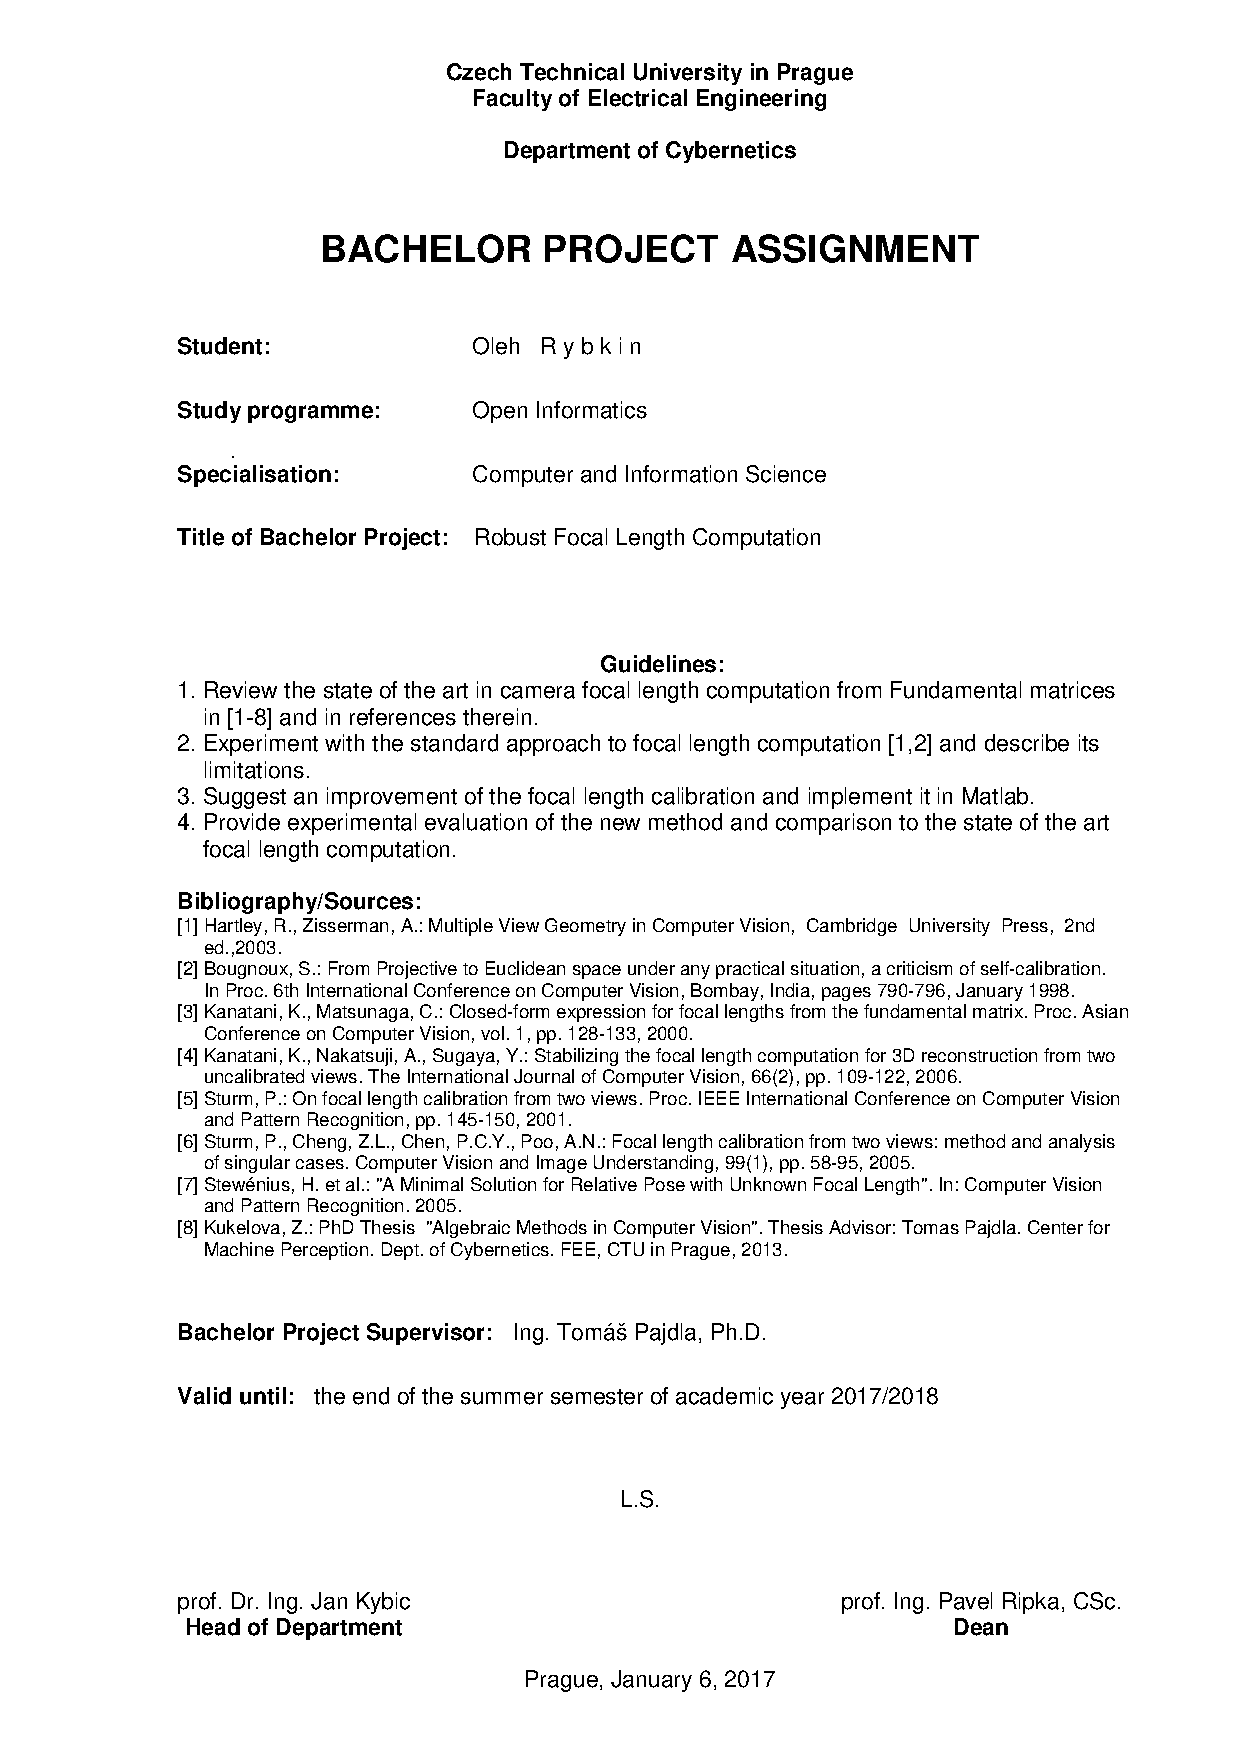
\includepdf[pages={1}]{assignment.pdf}

\cleardoublepage


\mbox{}\vfill

{\let\clearpage\relax\par \chapter*{Acknowledgements}}

I would like to thank my advisor Tomáš Pajdla for introducing me into the world of research and his numerous patient explanations of how things work and how the work is done. 
I would also like to thank Zuzana Kúkelová for precious comments and suggestions.

\endinput
\clearpage
\mbox{}\vfill

{\let\clearpage\relax\par \chapter*{Author's declaration}}
I declare that I have work out the presented thesis independently and that I have listed all information sources used in accordance with the methodical instructions for observing the ethical principles in the preparation of university theses.

{\let\clearpage\relax\par \chapter*{Prohl\'a\v sen\'i autora pr\'ace}}
Prohla\v suji, \v ze jsem p\v redlo\v zenou pr\' aci vypracoval samostatn\v e a \v ze jsem uvedl ve\v sker\'e pou\v zit\'e informa\v cn\'i zdroje v souladu s Metodick\'ym pokynem o dodr\v zov\'an\'i etick\'ych princip\r u p\v ri p\v r\'iprav\v e vysoko\v skolsk\'ych z\'av\v ere\v cn\'ych prac\'i.

\vskip3cm
\begin{tabular}{lp{1cm}c}
  V Praze dne \makebox[4cm]{\dotfill} &  & \makebox[5cm]{\dotfill}\\
  & & Podpis autora pr\'ace
\end{tabular}
\clearpage


\chapter*{Abstract}
The problem of automatically computing focal lengths of a pair of cameras from corresponding pair of images has long been a daunting task for 3D reconstruction  community. A number of methods were developed, but the commonly held view is that neither of them works good enough to be used in practical situations. We focus on the particular task of computing focal lengths from the point correspondences, which we deem to be the missing link for the problem solution.

We especially focus on existing algebraic solvers for computing the fundamental matrix and the Bougnoux formula for computing the focal lengths therefrom. We  survey these methods, as well as iterative methods \cite{HartleyPriors,Chandraker} proposed as their extensions,  and analyze their performance. Our results show that the number of imaginary estimates, as well as the error of the estimation, declines with growing number of correspondences used.  Moreover, based on our analysis we suggest that the computation of the ratio of focal length $r= f_2 \slash f_1$ is more robust than
computation of $f_1$ or $f_2$ alone. We propose an improvement to the solver of~\cite{HartleyPriors} based on this suggestion.

We furthermore assess performance of the methods in  degenerate situations, and show that for bigger levels of noise the effect of the degeneracies significantly decreases. Specifically, the degenerate case of intersecting optical axes is shown to almost vanish for realistic levels of noise.

We finally analyze the problem of computing focal length from the theoretical standpoint of algebraic geometry, and give two new formulae for computing camera focal length from a fundamental matrix. We show that using the right of them might help to avoid a known degeneracy. Specifically, the degeneracy where the plane defined by the baseline and the optical axis of one camera is perpendicular to the plane defined by the baseline and optical axis of the other camera, and where Bougnoux~(\cite{Bougnoux}) formula fails can in some cases be avoided. The degeneracy reduces to the case where all three formulae fail.

\paragraph{Keywords:} computer vision, 3D reconstruction, minimal problems, focal length, Gr\"ob\-ner basis

\begin{otherlanguage}{czech}
\chapter*{Abstrakt}

Problém automatického výpočtu ohniskových vzdáleností dvou kamer z odpovídajících obrázků je stále obtížnou úlohou pro komunitu 3D rekonstrukce. Pro vyřešení tohoto problému byla navržena řada metod. Má se ale za to, že žadná z nich nefunguje natolik dobře, aby mohla být použita v praktické situaci. V této tezi se proto  zaměříme na úlohu výpočtu ohniskové vzdálenosti z korespondencí v obrázku, kterou považujeme za chybějící článek pro vyřešení problému.

Zejména se zaměříme na existující algebraické solvery pro výpočet fundamentální matice, a na Bougnouxův vzorec, který z ní vypočte ohniskovou vzdálenost. Tyto metody prozkoumáme a zanalyzujeme jejich výkonnost. Ukážeme, že počet imaginárních odhadů, jakož i chyba odhadu ohniskové vzdálenosti klesají s rostoucím počtem použitých korespondencí. Rovněž zanalyzujeme degenerace metod a jejich efektivitu v degenerovaných situacích, stejně jako výkon existujících iteračních solverů~\cite{HartleyPriors, Chandraker}, a navrhneme zlepšení solveru {~\cite{HartleyPriors}}.

Dále provedeme analýzu problému výpočtu ohniskové vzdálenosti z hlediska algebraické geometrie. Ukážeme, že kromě Bougnouxova vzorce existují další dva vzorce pro výpočet ohniskové vzdálenosti kamery z fundamentální matice. Ukážeme, že použitím spravného z těchto vzorců se můžeme v některých případech vyhnout známé degeneraci. Konkrétně takové, kde rovina definovaná baselineou a optickou osou jedné kamery je kolmá na rovinu definovanou baselineou a optickou osou druhé kamery, a kde Bougnouxův vzorec ~\cite{Bougnoux} selhává. Degenerace se redukuje na případ, kdy selhávají všechny tři vzorce.

\paragraph{Klíčová slova:} počítačové vidění, 3D rekonstrukce, minimální problémy, ohnisková vzdálenost, Gr\"obnerovy báze
\end{otherlanguage}

\endinput
\clearpage
\cleardoublepage\def\thepage{\arabic{page}}\setcounter{page}{1}
\tableofcontents\pagestyle{headings}


\listoffigures

%\listofalgorithms

\glsaddall
\printglossary[type=\acronymtype,title=List of Symbols and Abbreviations]
\printglossary






\chapter{Introduction}
\section{Motivation}
We analyze the problem of computing epipolar geometry of two partially calibrated cameras, where only the focal lengths are unknown.

Estimating epipolar geometry with unknown focal lengths is an important issue in practical problems. In the laboratory environment it is possible to calibrate the camera beforehand using established procedures~\cite{HartZiss}. When taking images in the wild, however, it is often impractical or impossible to use these procedures. It is desirable to have an automated procedure to estimate camera calibration from images themselves. 

The usual way~\cite{bundler,colmap,openMVG} to estimate camera external and internal parameters is to extract points of interests~\cite{SURF,SIFT} with tentative correspondences, and use RANSAC~\cite{USAC} method for joint estimation of correspondence inlier pairs and camera parameters. In RANSAC, a procedure to compute camera parameters from a (preferably small) number of points is needed. These procedures, that essentially are used as black box in RANSAC, are called minimal problems because it is desirable to find a procedure that would use the theoretical minimum number of correspondences.

The basic procedure to compute the focal lengths and epipolar geometry given correspondences consists of two steps: finding a fundamental matrix and decomposing the matrix into calibration matrices and essential matrix. For the first task, the minimal needed number of correspondences is 7. Hartley and Zisserman~\cite{HartZiss} describe an algorithm for this which uses 7 correspondences as well as the singularity condition. The algorithm gives three different estimations of the matrix, i.e. one correct and two false ones. Hartley~\cite{HartleyDefense} also summarizes an  algorithm by Longuet-Higgins~\cite{Higgins} which uses 8 correspondences instead. Bougnoux~\cite{Bougnoux} gives a concise formula to compute focal length from the fundamental matrix, if the rest of calibration information, i.e., the principal point, the skew, the ratio of the pixel dimensions, is known.

The procedure suffers from a number of known failure cases:
\begin{itemize}
    \item It is not possible to determine a fundamental matrix if the correspondences are in singular position.
    \item The camera pair may have intersecting (or parallel) optical axes. In that case it is impossible to determine the focal lengths.
    \item The plane defined by the baseline and the optical axis of one camera may be perpendicular to the plane defined by the baseline and optical axis of the other camera. In this case no focal length can be recovered as the Bougnoux formula fails.
    \item All computed fundamental matrices may have rank 1 or be complex. 
    \item A computed focal length may be complex.
    \item There may be no such computed camera configuration where most points in 3D space lie in front of the cameras.
\end{itemize}

Because of these deficiencies, the commonly held view is that the algebraic approach of using 7pt algorithm and Bougnoux formula is not robust, and sometimes fails entirely, unable to find any valid solution. Hartley~\cite{HartleyPriors} argues that in many practical cases this approach cannot be used. Other methods~\cite{HartleyPriors,CNN,KanataniSub} were proposed to solve this problem. Neither of these approaches, however, works decisively better.

We analyze the procedure of computing focal lengths from points correspondences and different degeneracies to show that slight modifications of the procedure allow to alleviate a number of the problems.


\section{Related work}
Hartley and Silpa-Anan~\cite{HartleyPriors}  develop an iterative algorithm which incorporates heuristic estimates (prior knowledge) of focal lengths. The authors use optimization  on a certain cost function which includes the Sampson error, priors of focal lengths and priors of principal points.  They show that by allowing the algorithm to move principal point better results can be obtained. 
The algorithm shows competitive, although not decisively better performance in comparison to 7pt approach. In this thesis, we propose an improvement to this algorithm and demonstrate better performance.

Chandraker~\cite{Chandraker} further explores the idea of using priors of focal lengths. He defines a simpler cost function, and uses epipolar constraints as hard constraints, instead of including Sampson error in the cost function. The work considers two same focal lengths, but the algorithm can be easily extended to incorporate two focal lengths. 

Nakatsuji et al.~\cite{Kanatani3} show that even when the two focal lengths are the same, the 7pt algorithm (which assumes they are different) yields better accuracy than methods which assume the same focal length.
When the 7pt algorithm with the Bougnoux formula fail to produce a real focal length, he authors use 'subsampling' procedure. Points are subsampled from the set of inliers and the focal length is recomputed  each time from the sample until a real focal length is found.

Kanazawa et al.~\cite{KanataniSub} use three views for computing camera parameters (only two-view correspondences are needed for the method). Exploiting three different view pairs they are able to give more stable results than two-view methods.

DeepFocal, a recent algorithm by Scott Workman et al.~\cite{CNN}, uses a Convolutional Neural Network to estimate the focal length directly from one image. The neural network outperforms other approaches based on one view. While an interesting and fresh idea, authors didn't compare DeepFocal to any existing two-view approaches, therefore it is difficult to assess the advantages of the work.

\section{Thesis structure}


Our contributions are presented in Chapters~\ref{seq:analysis}, \ref{seq:algeom} and \ref{seq:thenew}.

In Chapter~\ref{seq:basic} we survey the basic concepts and establish notation for the thesis. In  Chapter~\ref{seq:analysis} we provide an analysis of the known methods for focal length computation and show their performance. In  Chapter~\ref{seq:algeom} we use algebraic geometry to further analyze the problem. In  Chapter~\ref{seq:thenew} we suggest improvements to the current methods using our analysis from  Chapter~\ref{seq:analysis}. We also provide a survey of methods that use prior focal length information.


\chapter{Basic notions}

\label{seq:basic}

\section{Camera geometry}

\begin{figure}[t]
  \begin{center}
    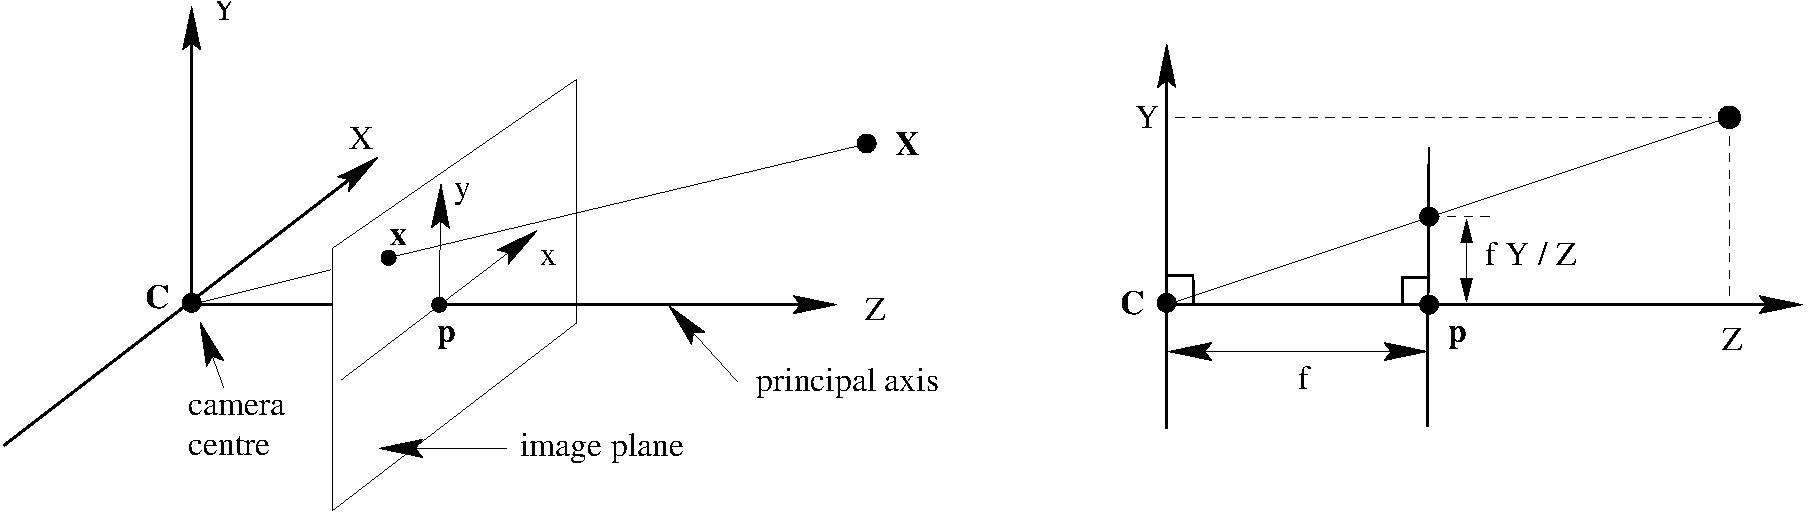
\includegraphics[width=\linewidth]{cammodel.pdf}
    \caption[Projective camera model]{Projective camera model. Courtesy of~\cite{HartZiss}}
    \label{cameramodel}
  \end{center}
\end{figure}

The book~\cite{HartZiss} describes camera geometry, the main topic of this thesis, in chapter 6. All needed preliminaries are also well described in chapters 1-5 of the book. In the next two sections we very briefly summarize and recapitulate the topic. We follow the notation of~\cite{HartZiss}.

\subsection{Single camera geometry}

The most convenient way of representing points in 3D or 2D space while dealing with camera geometry is using corresponding projective spaces.

\begin{defn}
Given a linear vector space $\R^n$, a \textit{projective space} $\Proj^{n-1}$ could be defined as a factorization of the linear space by a relation $\sim$: \[\mathbf{x}_1 \sim \mathbf{x}_2 \iff (\exists \lambda \in \R\backslash\{0\} \; \mathbf{x_1}=\lambda \mathbf{x_2}).\]

The zero point is also excluded from projective space.
\end{defn}


A point $\mathbf{X}_i=\mat{ccc}{x & y & z}^\T$ from 3D linear space $\mathbb{R}^3$  can be though of as a point $\mathbf{X}'=\mat{cccc}{x & y & z & 1}^\T$ from 3D projective space $\Proj^3$. Similarly, a point $\mathbf{X}'=\mat{cccc}{x & y & z & f}^\T$ can be converted back to the point $\mathbf{X}=\mat{ccc}{\frac{x}{f} & \frac{y}{f} & \frac{z}{f}}^\T$ unless $f$ is zero. Because of this possible conversion we will frequently refer to the same geometrical point as belonging to projective space $\Proj^{n-1}$ as well as linear space $\R^n$ simultaneously. 

\begin{defn}
A projective line is a line of points in projective space $\Proj^{n}$. Conveniently, it can be also represented by a point from the space  $\Proj^{n}$. For example, a line in projective plane $a x + b y + f c = 0$, which corresponds to the line $a x + b y + c = 0$ in  real plane, can be written as a point $\mathtt{l} = \mat{ccc}{a & b & c}^\T$.
\end{defn}


The Fig. \ref{cameramodel} shows an essential concept of projecting points from world (3D) space to image (2D) space. This projection can be described as a linear operation in corresponding projective spaces. 

The projection operator is given by camera parameters, which can be divided in two groups - extrinsic and intrinsic parameters.
We next define essential intrinsic parameters. 

\begin{defn}
\textit{The principal axis}, also \textit{optical axis}, is the line passing through camera center and perpendicular to the image plane.
\end{defn}

\begin{defn}
\textit{The principal point} $\mathbf{p}=\mat{ccc}{p_x & p_y & 1}^\T$ is the point lying at the intersection  of image plane and principal axis.
\end{defn}

\begin{defn}
\textit{The focal length} $f$ is the distance from the camera center to the principal point. 
\end{defn}

Camera intrinsic parameters are can be formed into camera calibration matrix.

\begin{defn}
\textit{A iatrix\footnote{Throughout this work we assume unity aspect ratio and zero skew.}} $\mathtt{K}$ is a matrix of the form \[ \mathtt{K} = \mat{ccc}{f & 0 & p_x \\ 0 & f & p_y \\ 0 & 0 & 1}. \] 
\end{defn}

If we assume that the camera center is the world space zero point, principal axis coincide with $Z$ axis, and image space axes $x$, $y$ are aligned with world space axes $X$, $Y$ (true for the Fig. \ref{cameramodel}), we can project 3D points with only camera intrinsics. The projection from $\R^3$ to $\Proj^2$ image plane is given by $\mathbf{x}_i = \mathtt{K} \mathbf{X}_i $.

Extrinsic parameters of a camera $i$ are described by a rotation matrix in the world space $\mathtt{R}_i$ describing camera orientation and the camera center point  $\mathbf{C}_i$ in the world space.  
Given extrinsic and intrinsic parameters, we can construct the full projection matrix.

\begin{defn}
The camera \textit{projection matrix} $\mathtt{P}_i$ can be constructed from camera parameters and projects points $\mathbf{X}_i$ from world space $\Proj^3$ to the image plane $\Proj^2$: \[\mathbf{x}_i = \mathtt{P} \mathbf{X}_i =  \mathtt{K} \mathtt{R} [ \mathtt{I} | -\mathbf{C} ] \mathbf{X}_i \].

\end{defn}


\subsection{Epipolar geometry} 
Epipolar geometry, one of the key topics of this thesis, is a geometry of two cameras seeing the same 3D object. 

This section is described in depth in chapter 9 of~\cite{HartZiss}. As a slight deviation from the notation of Hartley and Zisserman, cameras and respective image points are indexed with numbers, e.g., $\mathbf{x}_1$, $\mathbf{x}_2$ and not $\mathbf{x}$, $\mathbf{x}'$ respectively.


\begin{figure}[t]%
    \centering
    \subfloat{{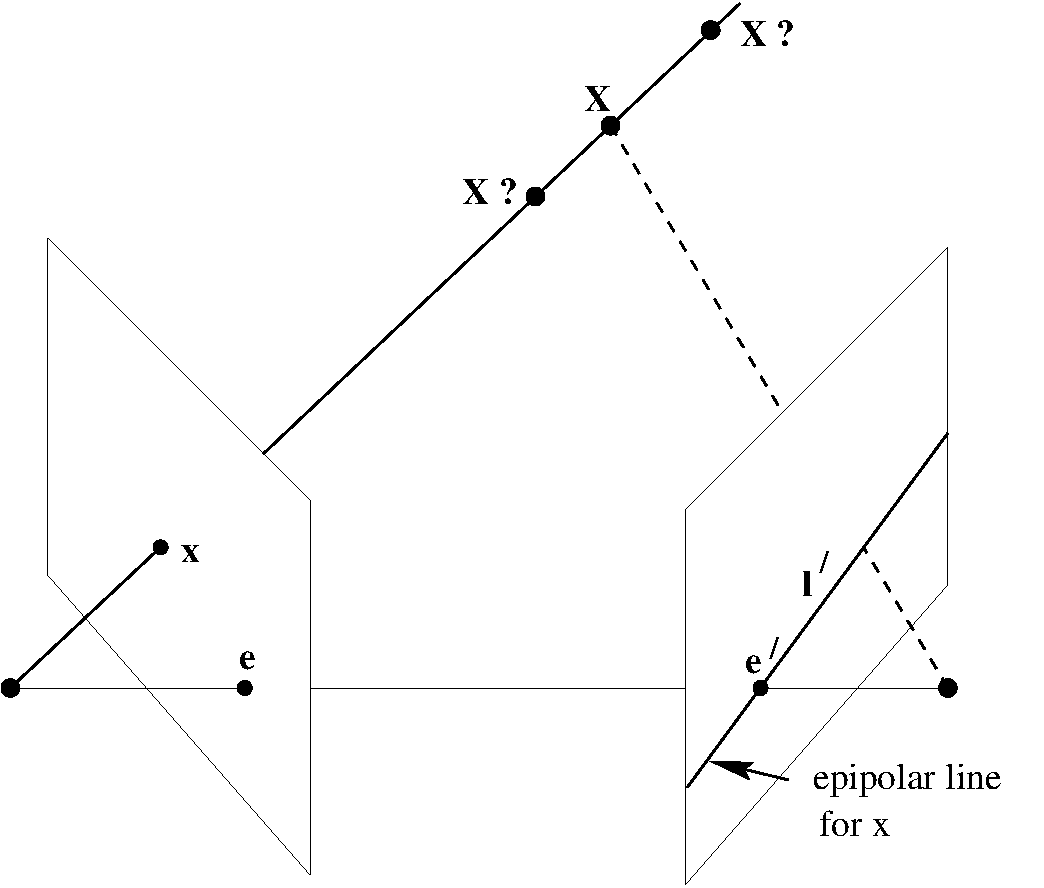
\includegraphics[width=5cm]{campair1.pdf} }}%
    \qquad
    \subfloat{{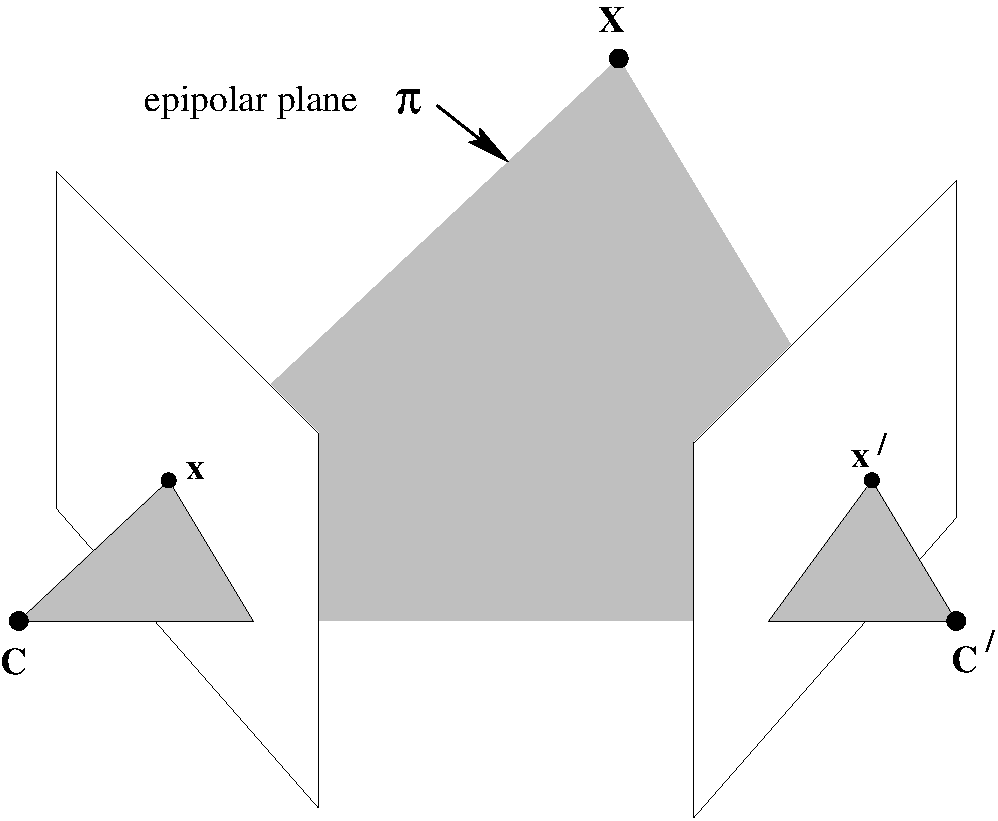
\includegraphics[width=5cm]{campair2.pdf} }}%
    \caption[Camera pair]{Camera pair. Courtesy of~\cite{HartZiss}}%
    \label{fig:campair}%
\end{figure}

Extrinsic parameters of a camera pair can be concisely given by the translation vector between camera centers $\mathbf{t}= \mathbf{C}_1-\mathbf{C}_2$ and the rotation matrix between cameras' coordinate systems $\mathtt{R}=\mathtt{R}_2\,\mathtt{R}_1^T$. If $\mathtt{R}, \mathbf{t}$ are known, extrinsics $\mathtt{R}_1, \mathtt{R}_2, \mathbf{C}_1, \mathbf{C}_2$ are defined up to a projective transformation.

Geometry of two cameras and a point in the world space seen by both cameras is usually described in terms of epipoles, which are the key concept of epipolar geometry. 


\begin{defn}
\textit{The baseline} is the line in 3D joining two camera centers.
\end{defn}

\begin{defn}
\textit{The epipole} $\mathbf{e}_i$ is the point in image plane that lies at the baseline. Equivalently, it is the point to which the center of another camera projects. 
\end{defn}

\begin{defn}
\textit{An epipolar line} $\mathbf{l}$ is a line in image plane on which the epipole of that plane lies.
\end{defn}

\begin{defn}
\textit{An epipolar plane} $\mathbf{\pi}$ is a plane in the world space which contains the line joining camera centers. The plane is associated with two epipolar lines that it contains.
\end{defn}

The information about camera epipolar geometry can be described by a single matrix as defined next. If interested, see extended discussion and proofs in \cite{HartZiss}.

\begin{defn}
\textit{An essential matrix} $\mathtt{E}$ is a matrix of the form $ \mathtt{E} = \mathtt{R} \cross{\mathbf{t}}$. The essential matrix is defined up to overall scaling.
\end{defn}

As can be seen from its construction, an essential matrix can only be of rank 2. A weaker version of this constraint can be stated as the rank constraint: 
\begin{equation}
\det{\mathtt{E}} = 0.
\label{eq:rank}
\end{equation}

The two non-zero singular values of an essential matrix are equal. This constraint can be stated as the next matrix equation (also called the trace constraint):
\begin{equation}
2 \mathtt{E} \mathtt{E}^\T \mathtt{E} - \trace{(\mathtt{E} \mathtt{E}^\T)} \mathtt{E} = 0.
\label{eq:trace}
\end{equation}

The equations \ref{eq:rank} and \ref{eq:trace} together are called  Demazure polynomials~\cite{Demazure}.

Essential matrix does not capture intrinsic camera parameters. For this purpose, the fundamental matrix is used.

\begin{defn}
\textit{The fundamental matrix} $\mathtt{F}$ corresponding to an Essential matrix $\mathtt{E}$ is given by

\begin{equation}
\mathtt{F} = \mathtt{K}_2^{-\T} \mathtt{E} \mathtt{K}_1^{-1}. 
\label{eq:fundamental}
\end{equation}
 The fundamental matrix is, like the essential matrix, defined up to overall scaling.
\end{defn}

The fundamental matrix of a camera pair defines a specific mapping from points in one image to epipolar lines in another image. Suppose that given an image point $\mathbf{x}_1 \in \Proj^3$ and two cameras $\mathtt{P}_1$, $\mathtt{P}_2$, the line $\mathbf{C}_1 \mathbf{x}_1$ in world space  is projected by the second camera to the line $\mathbf{l}_2 \in \Proj^3$ in the second camera image space. Then we can obtain $\mathbf{l}_2$ by $\mathbf{l}_2=\mathtt{F} \mathbf{x}_1$

\begin{defn}
We say that a point in one camera $\mathbf{x}_1$ and a point in another camera $\mathbf{x}_2$ form a \textit{correspondence} if there exists a 3D point $\V{X}$ that projects to $\V{x}_1$ and $\V{x}_2$.
\end{defn}

For each correspondence $\mathbf{x}_1, \mathbf{x}_2$, the fundamental matrix satisfies the so-called Epipolar constraint:
\begin{equation}
\mathbf{x}_2^\T \mathtt{F} \mathbf{x}_1 = 0.
\label{eq:epipolar}
\end{equation}

As with essential matrices, a fundamental matrix can only be of rank two. On the other hand, every matrix of rank two is a fundamental matrix~\cite{HartZiss}. A fundamental matrix satisfies the rank constraint
\begin{equation}
\det{\mathtt{F}} = 0.
\label{eq:rankF}
\end{equation}

A version of trace constraint on fundamental matrix can be formulated by substituting equation \ref{eq:fundamental} into equation \ref{eq:trace}.

\section{Computing focal lengths from point correspondences}
Given a set of points in one image $X_1$ and a set of points in another image $X_2$ that correspond to the same points $X$ in the world space, it is possible in some cases to determine the positions of points $X$ as well as intrinsic and extrinsic parameters of both cameras. This section guides the reader through the process.

Note, that in this part we assume that the point correspondences are given to us by a black box algorithm. In fact, many algorithms and modifications thereof were developed to this end, the most notable being the RANSAC family of algorithms~\cite{ransac}.


\subsection{Fundamental matrix computation}

First, we need to estimate the fundamental matrix $\mathtt{F}$ of a camera pair. In fact, all the information we need is contained in this matrix. 
Various algorithms exist that can compute the matrix $\mathtt{F}$ from point correspondences. We present two methods that are, to our best knowledge, used the most. They are relatively simple and can be implemented efficiently. 

The algorithms which we present can be formulated as so-called algebraic solvers, which work by way of constructing a set of constraints on the matrix $\mathtt{F}$ given the correspondences, and then solving the constraints in an algebraically precise way, giving all possible solutions. If the constraints are represented by polynomial equations the techniques of algebraic geometry can be used to solve these constraints.

We first define the 7pt algorithm. The algorithm uses (at least) 7 different epipolar constraints~\ref{eq:epipolar} and the rank constraint~\ref{eq:rankF}. This gives us 8 constraints on a 3$\times$3 matrix. Note, however, that all of the constraints are homogeneous polynomials, and thus the solution to the system will be a finite number\footnote{We suppose that the constraints are algebraically independent. Equivalently, at least 7 of the correspondence point pairs are in general position.} of linear one-dimensional spaces of matrices. As a fundamental matrix is defined up to scaling, this corresponds to a finite number of fundamental matrices. Moreover, the number of matrices can be expected to be no more than 3\footnote{This number is calculated as the product of degrees of the polynomials entering the system, which is  $3 \cdot 1^7$.}.

The algorithm uses SVD procedure which serves as an implicit optimization of the epipolar constraints. In case that precisely 7 epipolar constraints are given, SVD can be replaced with Gauss-Jordan elimination, and the $\mathbf{f}_1$, $\mathbf{f}_2$ vectors will be a basis of  right null space of the matrix $\mathtt{B}$. Equivalently, the matrices $\mathtt{F}_1$, $\mathtt{F}_2$ will be a basis of the pace of matrices that satisfy seven epipolar constraints.

\begin{algorithm}[H]
\SetAlgoLined 
\LinesNotNumbered
 \KwData{list of $n \geq 7$ right image points $\mathbf{x}_{1,i}$, list of the corresponding left image points $\mathbf{x}_{2,i}$}
 \KwResult{Fundamental matrix $\mathtt{F}$}
 \Begin
    {Populate matrix $\mathtt{B} \in \mathbb{R}^{n \times 9}$ with columns $\mathbf{b}_i$:  $\mathbf{b}_i \leftarrow  \vect(\mathbf{x}_{2,i} \kronecker \mathbf{x}_{1,i})$\; 
    
    Take the right singular vectors $\mathbf{f}_1, \mathbf{f}_2$ corresponding to the two smallest singular values and transform them back to matrices $\mathtt{F}_1, \mathtt{F}_2 \in \mathbb{R}^{3 \times 3}$ \;
    
    \eIf{$\det(\mathtt{F}_2)=0$}{
    \Return{ $\mathtt{F}_2$\;}
    }{
    Solve the 3rd degree polynomial in $x$: $\det(x \mathtt{F}_1 + \mathtt{F}_2)=0$, and choose the real roots $x_i$.\;
    
    \Return{ $x_i \mathtt{F}_1 + \mathtt{F}_2$\;}}
    }
 \caption{7pt}
 \label{7pt}
\end{algorithm}

Note, that we call this algorithm 7pt because the minimal number of correspondences it needs is 7. Nevertheless, any  number bigger than 7 can also be used. No smaller number of correspondences can be used, however. It can be proven that the problem  of computing fundamental matrices  with two unknown focal lengths is inherently ill-posed when less than 7 correspondences are given. The algorithm thus solves the problem using minimal possible number of correspondences.

The second algorithm doesn't use the rank constraint~\ref{eq:rankF}. Therefore, generically we expect the result to be a matrix of rank 3 and not a valid fundamental matrix. The matrix, however, "better" satisfies the epipolar constraints~\ref{eq:epipolar}, that is, it is more loyal to the data. We will compare the performance of this algorithm to 7pt in the later parts of the work. Note that this algorithm gives precisely one real solution.

\begin{algorithm}[H]
\SetAlgoLined 
\LinesNotNumbered
 \KwData{list of $n \geq 8$ right image points $\mathbf{x}_{1,i}$, list of the corresponding left image points $\mathbf{x}_{2,i}$}
 \KwResult{Fundamental matrix $\mathtt{F}$}
 \Begin
    {Populate matrix $\mathtt{B} \in \mathbb{R}^{n \times 9}$ with columns $\mathbf{b}_i$:  $\mathbf{b}_i \leftarrow  \vect(\mathbf{x}_{2,i} \kronecker \mathbf{x}_{1,i})$\;
    
    Take the right singular vector $\mathbf{f}$ corresponding to the smallest singular value and transform it back to matrix $\mathtt{F} \in \mathbb{R}^{3 \times 3}$ \;
    
    \Return{ $\mathtt{F}$\;}
    }
 \caption{8pt}
 \label{8pt}
\end{algorithm}

Note, that we call this algorithm 8pt because the minimal number of correspondences it needs is 8. Nevertheless, any  number bigger than 8 can also be used. 

\subsection{Essential matrix computation}
\label{sec:5pt}
If all calibration information is known, we can estimate essential matrix $\mathtt{E}$ instead of $\mathtt{F}$. This can be done by transforming points so that effects of intrinsic camera parameters are removed: \[\tilde{\mathbf{x}}_i = \mathtt{K}_i^{-1} \mathbf{x}_i. \]

Then the epipolar constraint \ref{eq:epipolar} is satisfied by the essential matrix with respect to the transformed points: \[
\tilde{\mathbf{x}}_2^\T \mathtt{E} \tilde{\mathbf{x}}_1 = 
 \mathbf{x}_2^\T \mathtt{K}_2^{-\T} \mathtt{E} \mathtt{K}_1^{-1} \mathbf{x}_1 = \mathbf{x}_2^\T \mathtt{F} \mathbf{x}_1 = 0. \]

The algebraic solver for the essential matrix uses the rank constraint \ref{eq:rank}, the trace constraint \ref{eq:trace}, and needs 5 point correspondences. Note that the trace constraint is a matrix equation, and therefore actually stands as more than one constraint, which explains why counting degrees of freedom seemingly fails in this case.

The construction of the solver is considerably more involved than the previous algorithms, therefore we will only refer to the papers that describe it fully.

Nister et al.~\cite{Nister5pt} show in detail how to construct an algebraic solver for this problem. The paper makes extensive use of theory of algebraic geometry \cite{Cox1,Cox2}. It is very instructing to read through the construction of this solver.

We will, however, use another solver, described by Kukelova et al. in~\cite{Zuzana5pt}. The code can be found online at \hyperref[http://cmp.felk.cvut.cz/mini/]{''http://cmp.felk.cvut.cz/mini/''}\footnote{Enter 'Polynomial eigenvalue solutions to minimal problems in computer vision' in the search field.}. This solver, contrary to the one by Nister et al., makes it possible to use an arbitrary number of correspondences, which we will take advantage of. We will refer to this solver as \textit{5pt solver}.

For those interested, Kukelova et al. give an algorithm (with source code) that  automatically creates solvers for algebraic problems~\cite{generator}.


\subsection{Focal lengths computation}
Bougnoux~\cite{Bougnoux} gives a concise formula to compute focal length from the fundamental matrix, if principal point position is known. In the next two formulae the matrix $\mathtt{I}_2$ is defined as $\mathtt{I}_2=\diag(1,1,0)$, and $\mathbf{e}_1, \mathbf{e}_2$ are the epipoles of the first and second image correspondingly. 
\begin{equation}
\label{eq:bougnoux1}
f^2_1=-\frac{\mathbf{p}^\T_2 \cross{\mathbf{e}_2} \mathtt{I}_2 \mathtt{F} \mathbf{p}_1 \mathbf{p}^\T_1 \mathtt{F}^\T \mathbf{p}_2}{\mathbf{p}^\T_2 \cross{\mathbf{e}_2} \mathtt{I}_2 \mathtt{F}^\T \mathtt{I}_2 \mathtt{F} \mathbf{p}_2}
\end{equation}

\begin{equation}
\label{eq:bougnoux2}
f^2_2=-\frac{\mathbf{p}^\T_1 \cross{\mathbf{e}_1} \mathtt{I}_2 \mathtt{F}^\T \mathbf{p}_2 \mathbf{p}^\T_2 \mathtt{F} \mathbf{p}_1}{\mathbf{p}^\T_1 \cross{\mathbf{e}_1} \mathtt{I}_2 \mathtt{F} \mathtt{I}_2 \mathtt{F}^\T \mathbf{p}_1}
\end{equation}

The second equation may be derived from the first by switching indices and transposing the $\mathtt{F}$ matrix. 

Note that it is not possible to find a focal length unless both principal points are known. As these formulae show, generically, the focal lengths are different for different principal point positions.

\subsection{Failure cases}
\label{seq:failure}
We consider the failure cases  that may occur while estimating focal length using 7pt algorithm and the Bougnoux formula.

\subsubsection{Degeneracies}
The first possible degeneracy is that the 7 epipolar constraints~\ref{eq:epipolar} are \textit{linearly dependent}. This means that the system is underconstrained and there will be generically an infinite number of solutions. A configuration of 7 correspondences which lead to such a system is said to be in singular position.

Agarwal et al., in a thorough study \cite{OnExistence}, analyze by algebraic geometry techniques a degeneration when neither of 3 solutions that 7pt algorithm gives are actually valid Fundamental matrices. It is shown in the paper that meeting the rank constraint is not enough for a matrix to be a fundamental matrix, as it needs to be of rank precisely 2. There may be a degeneracy when the matrix \textit{is of rank 1}\footnote{We suppose that algorithm does not return zero solution $\mathtt{F}=0_{3,3}$. Our formulation of the 7pt algorithm indeed does not naturally produce this solution.}. However, the constraint "is not of rank 1" cannot be expressed algebraically in an easy way and doesn't reduce the number of degrees of freedom of $\mathtt{F}$, as it only affects an infinitely small fraction of matrices. The preferable way of dealing with this degeneracy is thus to select only the valid subset of the 3 solutions given by the 7pt algorithm.

Another degeneracy may occur when the camera pair has \textit{intersecting (or parallel) optical axes}. In that case it is impossible to determine the focal lengths~\cite{KanataniClosed}. We now formulate a concise condition which describes when this can happen.

\begin{lem}
Optical axes of cameras $\mathtt{P}_1, \mathtt{P}_2$ as lines in projective $\Proj^3$ space intersect\footnote{In projective space we say that two parallel lines intersect at a point at infinity.} if and only if the principal points $\mathbf{p}_1$, $\mathbf{p}_2$ satisfy the epipolar constraint \begin{equation*}
      \mathbf{p}_2^\T \mathtt{F} \mathbf{p}_1 = 0.
\end{equation*} 

Moreover, if the principal points are zero points $\mathbf{p}_1=\mathbf{p}_2=\mat{ccc}{0 & 0 & 1}^\T$, the optical axes intersect if and only if the rightmost lowest element of the corresponding fundamental matrix $\mathtt{F}$ is zero \[ \mathtt{F}_{3,3} = 0\].
\label{interlemma}
\end{lem}

\begin{proof}
 The first part. If optical axes intersect, the point at their intersection is projected to images' principal points. Thus, principal points form a correspondence and must satisfy the epipolar constraint. Conversely, if the principal points satisfy the epipolar constraint, they must lie in an epipolar plane (see Fig. \ref{fig:campair}). The optical axes are then also lying in the epipolar plane, and each two projective lines in a plane intersect.
 
 The second part. Consider the following: \[ \mathbf{p}_2^\T \mathtt{F} \mathbf{p}_1 = \mat{ccc}{0 & 0 & 1} \mat{ccc}{
 \mathtt{F}_{1,1} & \mathtt{F}_{1,2} & \mathtt{F}_{1,3} \\ \mathtt{F}_{2,1} & \mathtt{F}_{2,2} & \mathtt{F}_{2,3} \\ \mathtt{F}_{3,1} & \mathtt{F}_{3,2} & \mathtt{F}_{3,3}}
 \mat{ccc}{0 \\ 0 \\ 1} = \mat{ccc}{0 & 0 & 1} \mat{ccc}{\mathtt{F}_{1,3} \\ \mathtt{F}_{2,3} \\ \mathtt{F}_{3,3}} = \mathtt{F}_{3,3}\]
\end{proof}

A further degeneracy \cite{HartZiss} occurs when  the plane defined by the baseline and the optical axis of one camera \textit{is perpendicular} to the plane defined by the baseline and optical axis of the other camera. In this case the Bougnoux formulae have zero denominator and thus fail to estimate the focal lengths.

\subsubsection{Invalid solutions}
There are also cases when the matrix and the focal lengths can be computed but don't correspond to any real camera configuration.

Some solutions that may need to be filtered out are \textit{complex} $\mathtt{F}$ \textit{matrices}. In the 7pt algorithm, as we are solving a 3rd degree polynomial, we may end up with 2 complex and one real solution. This might be a problem if the real solution $\mathtt{F}$ is a matrix on rank 1, and thus we don't have any valid result.

Hartley shows in~\cite{HartleyPriors} that the focal lengths computed may be imaginary, which again leads to impossible camera configuration. This happens because the focal length enter the Bougnoux formulae (Eq.~\ref{eq:bougnoux1}) only squared, so a negative estimation of $f^2$ leads to a purely imaginary focal length and can occur even when all the coefficients are real. Hartley argues that this is unacceptable and addresses the problem by developing a new algorithm to find a matrix which will have a valid focal length. 

Another problem is described in conjunction with the notion of \textit{cheirality} in~\cite{Cheirality}. In the projective camera model, we allow the points from behind the camera to be projected to image plane. This introduces an ambiguity when decomposing the essential matrix into rotation and translation. Four different camera pairs can be constructed that will have the same essential matrix, corresponding to two possible orientations of each camera, one that has points in front of it and one that has points behind.

Normally, we are able to pick the right reconstruction by selecting the camera pair such that cameras have points in front of them in world space. However, with presence of large noise it can happen that no such camera pair will exist. Usually the configuration that has the points in front of it is chosen, but this strategy can produce a wrong configuration. 

%\section{Getting point correspondences}
%for joint estimation of correspondence inlier pairs and camera parameters.


\section{Algebraic Geometry}

This section serves as a brief introduction of the topic of algebraic geometry. We follow the notation of Cox et al. from \cite{Cox1}\cite{Cox2}. We refer an interested reader to these books. 

First we define the key algebraic object of the algebraic geometry.

\begin{defn}
Given a polynomial ring $\C[x_1,x_2, \dots, x_n]$, \textit{an ideal} $I$ is such a subset of the ring that is closed under addition as well as under multiplication by a polynomial from $ \C[x_1,x_2, \dots, x_n]$. Specifically,
\begin{align*}
  & \forall f_1,f_2 \in I \; : \;  f_1+f_2 \in I \\
  & \forall f \in I, h \in  \C[x_1,x_2, \dots, x_n] \; : \; h f \in I .  
\end{align*}
\end{defn}
We can generate a geometrical object from an ideal, as outlined in the next definition.

\begin{defn}
We define a function $\textbf{V}(I)=V$, where $I \subset \C[x_1,x_2, \dots, x_n]$, and $V \subset \C^n$. \[\textbf{V}(I)=\{ a \in \C^n \; | \; f(a) = 0 \text{ for all } f \in I \} \] Intuitively, $V$ is a set of solutions to a (possibly infinite) system of polynomial equations~$I$.
\end{defn}

The geometrical sets that can be constructed in such a way are called varieties.
\begin{defn}
\textit{A variety} $V$ is such a set $V \subset \C^n$ that $\textbf{V}(I)=V$ for some system of polynomial equations  $I \subset \C[x_1,x_2, \dots, x_n]$. 
\end{defn}

We can also generate an ideal back from a variety.
\begin{defn}
We define a function $\textbf{I}(V)=I$, where $V \subset \C^n$, and $I \subset$ \( \C[x_1,x_2, \dots, x_n]\). \[\textbf{I}(V) =  \{f \in \C[x_1,x_2, \dots, x_n] \; | \; f(a) = 0 \text{ for all } a \in V \}. \] Intuitively, $I$ is a maximal set of polynomial equations that determines the geometrical set $V$.
\end{defn}

A known result~\cite{Cox1} is that $\textbf{V}(\textbf{I}(V))=V$. Under a certain assumption\footnote{When the ideal concerned is a so-called radical ideal~\cite{Cox1}.}, the opposite is also true $\textbf{I}(\textbf{V}(I))=I$.

An important notion of Gr\"obner bases is somewhat analogical to linear bases from linear algebra. Defining Gr\"obner bases requires more involved terms, so we won't do it here. Instead, we state an important result, which offers an intuitive understanding of them. 
\begin{defn}
If $G$ is \textit{a Gr\"obner basis} $G=\set{g_1, g_2, \dots, g_m} \subset I$ of an ideal \\ $I \subset \C[x_1,x_2, \dots, x_n]$, then: \[ I = \langle g_1, g_2, \dots, g_m \rangle = \{  \sum_{i=1}^m h_i g_i \; | \;  h_1, h_2, \dots, h_m \in \C[x_1,x_2, \dots, x_n] \} \]
\end{defn}

An important result~\cite{Cox1} states that every ideal defined on a finite-dimensional polynomial ring has a finite Gr\"obner basis. Continuing the analogy with linear bases, a Gr\"obner basis of a set of polynomials of degree 1 (i.e., linear equations) system is indeed its linear basis.



\include{chapters/related}


\chapter{Experimental analysis of existing solutions}

\label{seq:analysis}

In this chapter we provide an assessment of the the quality and stability of the 7pt algorithm (algorithm~\ref{7pt}) with the Bougnoux formula (Eq.~\ref{eq:bougnoux1}). We consider this pipeline as essentially integral baseline procedure for estimation of the focal lengths from image correspondences.


\section{Experimental setup}


We assume zero skew and unity aspect ratio in both cameras and consider a partially calibrated problem, i.e., the principal points are known. We assume that the images were preprocessed in a way that principal points are always in the center. This means that the calibration matrices after this preprocessing are of shape \[ \mathtt{K}_i = \mat{ccc}{f_i & 0 & 0 \\ 0 & f_i & 0 \\ 0 & 0 & 1}. \] Different cameras are allowed to have different focal lengths.

\subsection{Evaluation procedure}
The setup for most experiments in the work is as follows:

\begin{algorithm}[H]
\SetAlgoNoLine
\LinesNumbered
 \KwData{The number of correspondences used $n$, noise $\sigma$}
 \Begin
    {Create a camera pair $\mathtt{P}_1$, $\mathtt{P}_2$ with focal lengths $f_1$,$f_2$\; 
 
    Create a point cloud $\mathtt{X} \in \mathbb{R}^{3 \times n}$ of $n$ points in 3D \;
    
    Project $\mathtt{X}$ to the cameras $\mathtt{P}_1$ and $\mathtt{P}_2$, producing the ground truth image point sets ${\mathtt{x}}_1^{gt}$, ${\mathtt{x}}_2^{gt} \in \mathbb{R}^{2 \times n}$ \;
    
    
    Apply additive noise drawn from $\mathcal{N}(0,\,\sigma^{2})$ to both $x$, $y$ coordinates of each point from ${\mathtt{x}}_1^{gt}$ and ${\mathtt{x}}_2^{gt}$. This produces observed image point sets $\mathtt{x}_1^{ob}$ and $\mathtt{x}_2^{ob}$ correspondingly \;
    
    Select 7 pairs of corresponding points $\mathtt{x}_1$ and $\mathtt{x}_2$, and let the remaining pairs to be the test set $\mathtt{x}_1^{test}, \mathtt{x}_2^{test}$ \;
    
    Get the $\mathtt{F}_i$ estimates of the fundamental matrix $\mathtt{F}$ from the correspondences $\mathtt{x}_1,\mathtt{x}_2$  (e.g. $i = 1\dots 3$ when using the 7pt algorithm (algorithm~\ref{7pt})). Leave only matrices with real elements\;
    
    %Choose the estimation that has the most support points from test set using the voting procedure\;
    Choose the estimation that optimizes Sampson error (equation~\ref{eq:sampson}) on the test set\;
    
    Estimate the focal lengths from the fundamental matrix $\mathtt{F}$ using the formulae~\ref{eq:bougnoux1} and \ref{eq:bougnoux2}\;
    }
 \caption{Workflow}
 \label{workflow}
\end{algorithm}

%The voting procedure allows to choose a fundamental matrix that fits data with big 

\subsection{Estimation quality measure}
\begin{figure}[h!]
      \begin{center}
    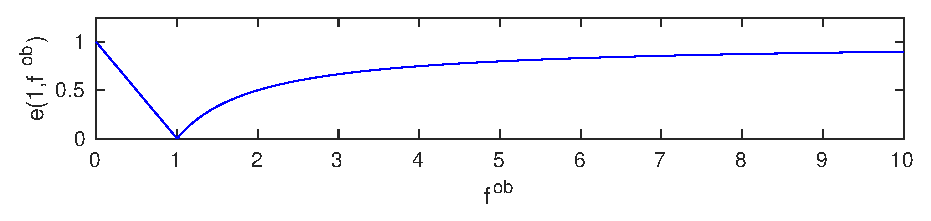
\includegraphics[width=\linewidth]{error_eval.eps}
    \caption[Focal length error function]{Error function \ref{eq:error} for the focal length, where $f_{gt}$ is fixed to 1.}
    \label{fig:error}
  \end{center}
\end{figure}
We treat error in focal length estimation as multiplicative, so that the error in case where the ground truth $f_{gt}=1000$ and computed value $f_{ob}=2000$ is the same as error in case where the ground truth $f_{gt}=100$ and computed value $f_{ob}=200$. More precisely the error is given by 
\begin{equation}
e(f_{gt},f_{ob})= 1 - \frac{\min(f_{gt}, f_{ob})}{\max(f_{gt}, f_{ob})}.
\label{eq:error}
\end{equation} The error function for fixed ground truth value $f_{gt}=1$ is shown in the Fig.~\ref{fig:error}.  

For measuring the quality of a fundamental matrix we use the Sampson error: 
\begin{equation}
S(\mathtt{F}) = \sum_i \frac{(\mathbf{x}_2^\T \mathtt{F} \mathbf{x}_1)^2}{(\mathtt{F} \mathbf{x}_1)_1^2 + (\mathtt{F} \mathbf{x}_1)_2^2 + (\mathbf{x}_2^\T \mathtt{F})_1^2 + (\mathbf{x}_2^\T \mathtt{F})_2^2}.
\label{eq:sampson}
\end{equation}


\section{Performance analysis for generic situations}

In this section we analyze the focal length computation performance for a generic scene, in which a degeneracy is unlikely to occur. 

In experiments, we each time generate a random set of points and a random camera pair so that the set of correspondences in each image span at least 1000 $\times$ 1000 pixel square. 


\subsection{Overall analysis}
We analyze the behavior of the pipeline against different numbers of given correspondences and different levels of noise. The quality of the estimation is assessed by computing the median of focal lengths computation  error $e$ and its 0.25 and 0.75 quantiles. In these experiments we discard each all imaginary estimates.

The Fig.~\ref{mean_v_corrs} shows a rapid decline in error with growing number of correspondences. This is explained by the fact that both algorithms use SVD procedure to optimize error on epipolar constraints. With bigger number of correspondences the error caused by random noise is averaged and the estimation becomes more stable. %Using 20 correspondences we can achieve an error close to negligible.
% This may be explained by the known fact that the 8pt solver optimizes error of matrix $\mathtt{F}$ in a certain sense \TP{Explain better. What do you mean by "certain sense"? What do you mean by "error of matrix"?}, as described by ? in~\cite{}. 

\begin{figure}[h!]
  \begin{center}
    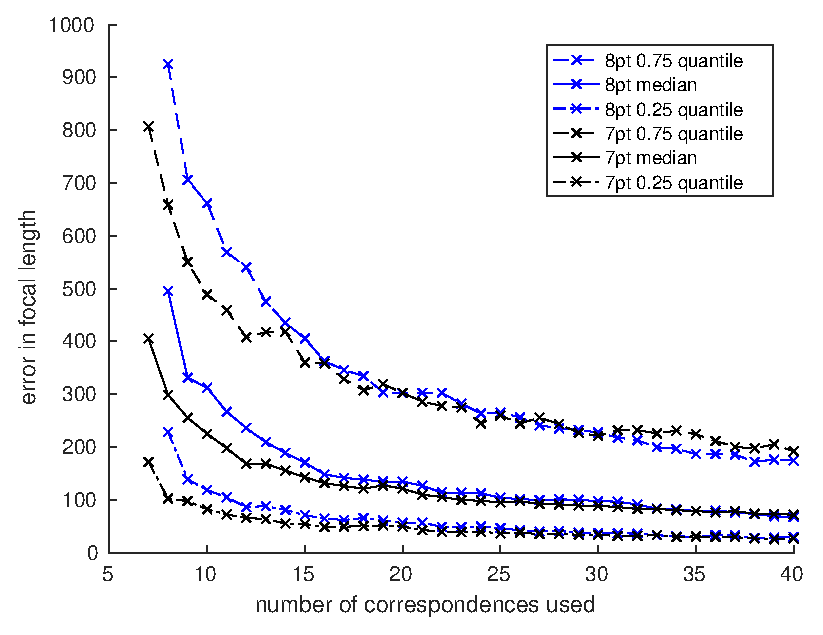
\includegraphics[width=\linewidth]{mean_error_corrs.eps}
    \caption[Error in focal length versus number of correspondences]{A Comparison of the 7pt and 8pt algorithms against the number of correspondences used. Median error $f - f^{true}$ in focal length and two its 0.25, 0.75 quantiles are shown. The ground truth $f^{true}$ is equal to 1500. The level of noise $\sigma$ is equal to 1. Imaginary estimates are excluded. }
    \label{mean_v_corrs}
  \end{center}
\end{figure}

The Fig.~\ref{mean_v_noise} shows the growth of the error with increasing noise. The number of  correspondences used is 8 for both algorithms. We see that the error growth is approximately linear and quite mild, e.g., with additive noise of 3 pixels the error is still bearable. For realistic values of noise around 1 pixel, the error is reasonably small.



\begin{figure}[h!]
  \begin{center}
    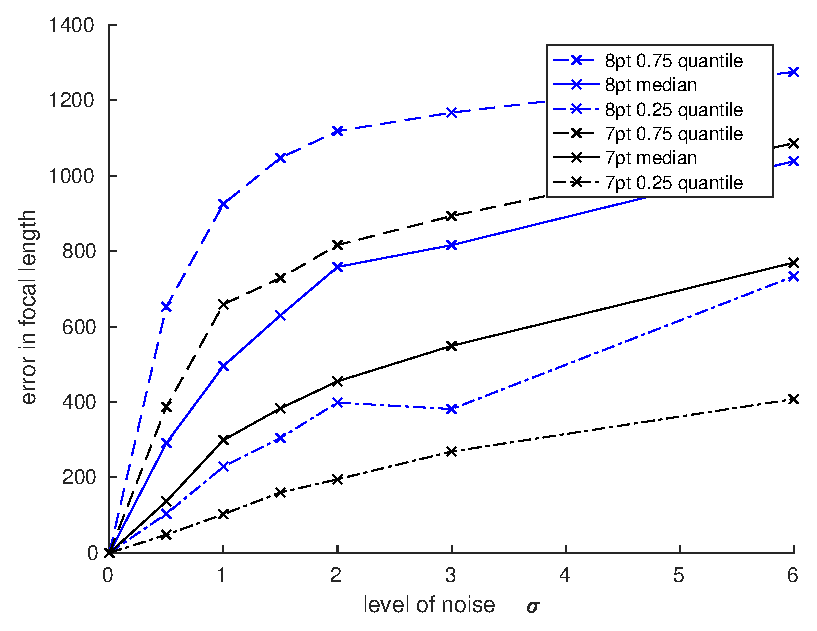
\includegraphics[width=\linewidth]{mean_error_noise.eps}
    \caption[Error in focal length versus level of noise]{A comparison of the 7pt and 8pt algorithms against noise level $\sigma$. The ground truth $f^{true}$ is equal to 1500. 40 correspondences are used.}
    \label{mean_v_noise}
  \end{center}
\end{figure}

Another important trend  is shown in the Fig.~\ref{imaginary_number} is the decrease of number of imaginary estimates with increasing number of correspondences used. We suggest that imaginary focal lengths are due to high level of noise, and appear less often when the noise is averaged over a  big number of correspondences.

\begin{figure}[h!]
  \begin{center}
    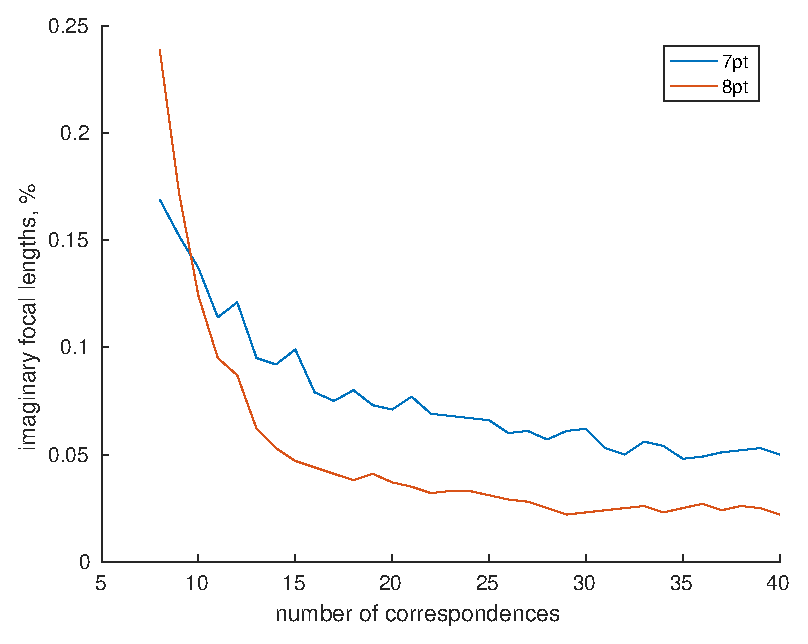
\includegraphics[width=\linewidth]{imaginary_number.eps}
    \caption[Fraction of imaginary focal length estimates versus number of correspondences]{The fraction of imaginary focal length estimates by the 7pt and 8pt algorithms. The noise level $\sigma$ in image measurements is equal to 1. }
    \label{imaginary_number}
  \end{center}
\end{figure}

We conclude that when the estimate of the focal lengths is real we can generally expect it to be quite precise and usable for most practical cases. More correspondences insure good performance, and moderate amounts of noise can be handled well. The 7pt algorithm performs better for most applications, however, interestingly enough, the 8pt algorithm gives less imaginary estimates.

\subsection{Ratio of focal lengths is robust}

We will continue to analyze the 7pt algorithm, as it apparently performs better than the 8pt algorithm on average. The 7pt algorithm also has the theoretical advantage in that it never gives a matrix of rank 3 (remember that a fundamental matrix is always of rank 2).


We  show empirically that the ratio $r={f_2}\slash{f_1}$  computation is more robust than computation of $f_1$ or $f_2$ alone.
To show it we conduct an experiment with  300 different noise samples applied to the same camera geometry. We exclude extreme outliers.

The Fig.~\ref{scatter} shows scattered estimated points in the space $(f_1,f_2)$. If the distribution of estimates in this space doesn't have additional structure, we expect these estimations to lie around the ground truth, perhaps similar to a two-dimensional Gaussian distribution. However,  it can be seen that while the deviation of focal lengths from the ground truth point is relatively big, the points clearly tend to the line $f_2 \slash f_1= 3\slash4$ (given in blue), which is indeed the ground truth for the ratio. Imaginary estimates are also shown in absolute values, which, interestingly, also tend to have the right ratio. We will expand on this in the next section.

We conclude that the computation of the ratio of the focal lengths $r$ by Bougnoux formula is more robust than the the computation of focal lengths themselves by the Bougnoux formula.
We will use this fact later to construct a more robust solver.

\begin{figure}[h!]
  \begin{center}
    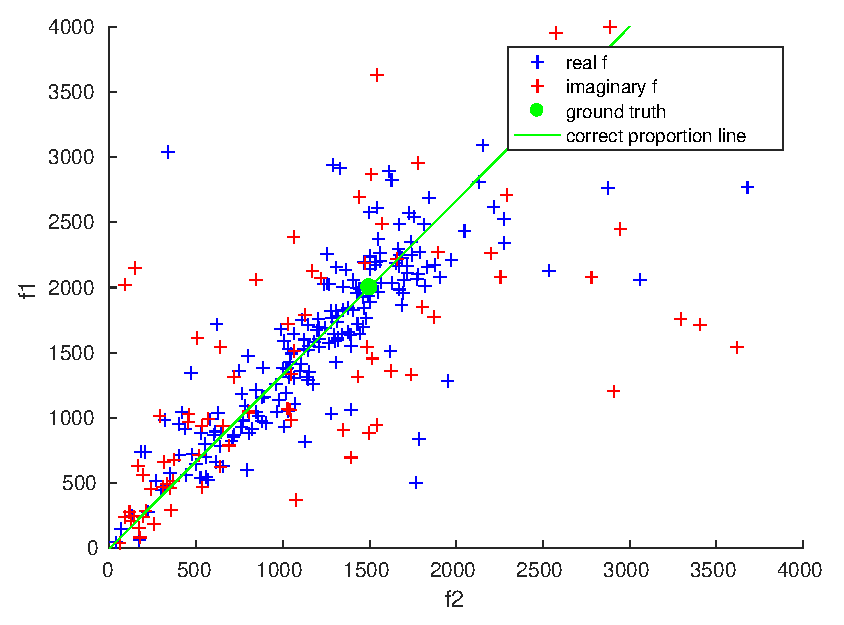
\includegraphics[width=\linewidth]{bougnoux_scatter.eps}
    \caption[Scattered focal length estimates]{The scatter plot of the focal lengths $(f_1, f_2)$ estimates by the 7pt algorithm for one scene. Line through ground truth ratio $r = f_2\slash f_1$ is given for reference. Ground truth point also shown in green. Imaginary estimates are shown in absolute value. The noise level $\sigma$ in image measurements in image measurements is equal to 1. Seven correspondences are used.}
    \label{scatter}
  \end{center}
\end{figure}

\subsection{Imaginary focal lengths}
\label{sec:Imaginary}
We empirically show that the ratio of the focal lengths is robust even when both focal lengths are imaginary.
The probability of getting an imaginary focal length also  isn't connected to distance between optical axes. 

Fig.~\ref{imagist_ratio} shows the experiment. The figure is the histogram of different errors in ratio (measured as $f_2\slash f_1-(f_2/f_1)_{gt}$).  A small number of outliers lies far off the graph.
Clearly, the likelihood that a focal lengths ratio is estimated better is bigger when the focal lengths are real. However, the Fig.~\ref{imagist_ratio} shows that the ratios  computed from imaginary focal lengths also fall reasonably close to the ground truth, in the sense that the mean of their distribution seem to converge to the ground truth ratio.

The distribution of the imaginary focal lengths itself is shown in the Fig.~\ref{imagist}. We see that for bigger values of error, the number of imaginary estimates is roughly equal to the number of real ones, in other words, the likelihood of getting an imaginary focal length estimate is around 50$\%$ when the error in focal length estimate is bigger than twofold. 

 We suggest that there is a hidden variable that is susceptible to noise and makes both focal lengths imaginary when the level of noise is high. It doesn't, however, affect the absolute values of the squares of the focal lengths. The variable seems to be selecting the sign of the square of the focal lengths in a way that the higher the noise is the more probable it is that the sign will be negative. 

 One of our guesses was that the probability of having imaginary estimate can increase when the situation becomes close the degenerate. In the next experiment we assess the degree of degeneracy by the length of shortest transversal between the optical axes. When the length is zero, the optical axes intersect. 

The Fig.~\ref{scatter_imaginary} shows the estimated ratios $r=f_2\slash f_1$. We see that the fraction of imaginary estimates does not depend on the length of shortest transversal. We also see how both ratios computed from real and imaginary estimates tend to the ground truth. We plot the ratios estimated from imaginary values of the focal lengths with negative sign and in red to distinguish it from the ratios estimated from the real values, which are shown in blue.


\begin{figure}[h!]
  \begin{center}
    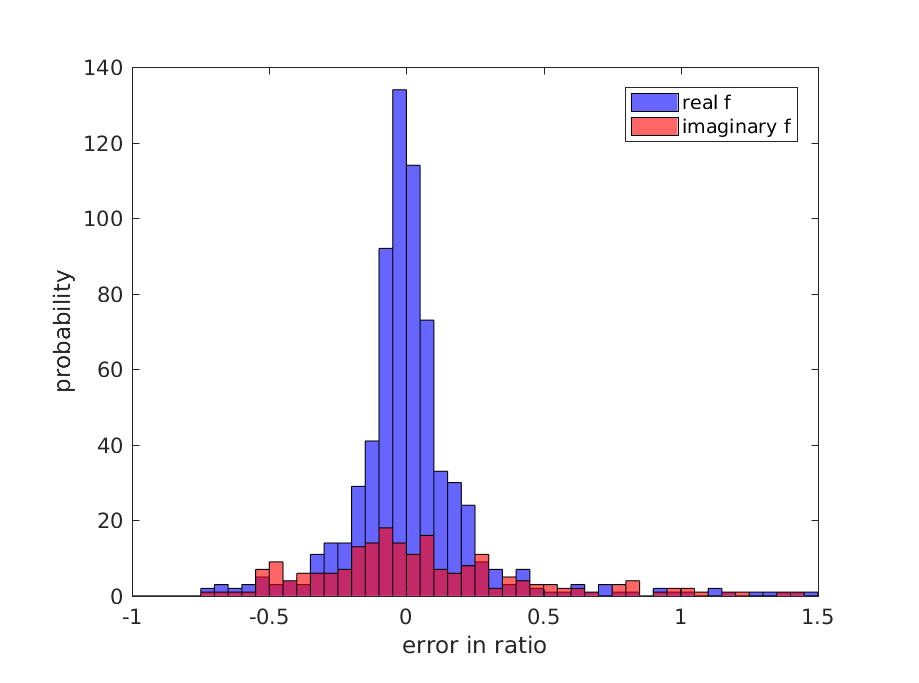
\includegraphics[width=\linewidth]{imaginary_hist_ratio.eps}
    \caption[Histogram of errors in the ratio of the focal length]{The histogram of errors in the ratio of focal length estimations by 7pt algorithm, i.e.\  $f_2 \slash f_1 - f_2^{true} \slash f_1^{true}$ . The cases with at least one imaginary focal length are shown in a separate histogram (orange), the cases where both focal length were real are shown in blue.  Red color is shown where an orange is supersimposed over blue. 40 correspondences are used, and level of noise $\sigma$ is equal to 1. A small number of outliers lies far off the graph.}
    \label{imagist_ratio}
  \end{center}
\end{figure}


\begin{figure}[h!]
  \begin{center}
    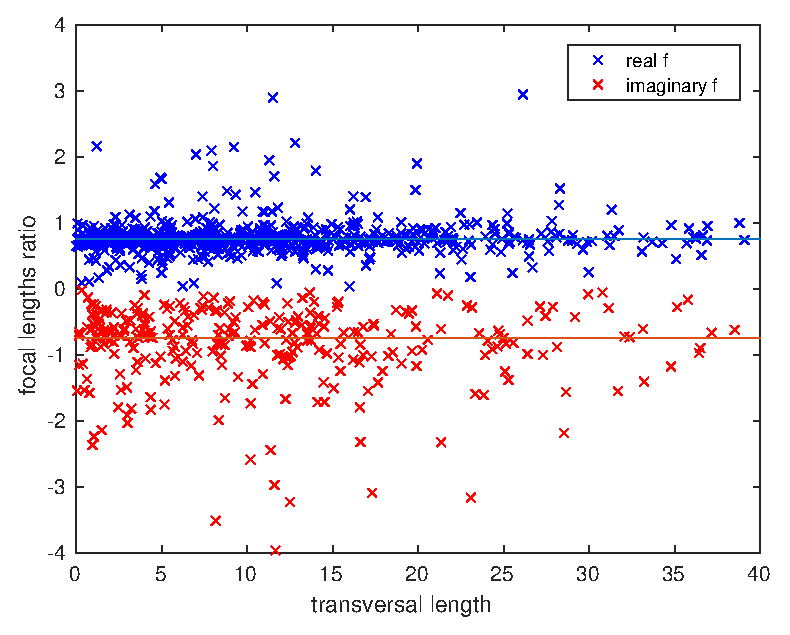
\includegraphics[width=\linewidth]{scatter_imaginary.eps}
    \caption[Scattered focal length ratio estimates]{Scatter plot of focal lengths ratio $r=f_2\slash f_1$ estimates produced by 7pt algorithm. Ratios corresponding to imaginary focal lengths are plotted as negative to distinguish them (they are positive). On $X$ axis is the distance between optical axes.  A small number of outliers lies far off the graph.. 40 correspondences are used. }
    \label{scatter_imaginary}
  \end{center}
\end{figure}

\begin{figure}[h!]
  \begin{center}
    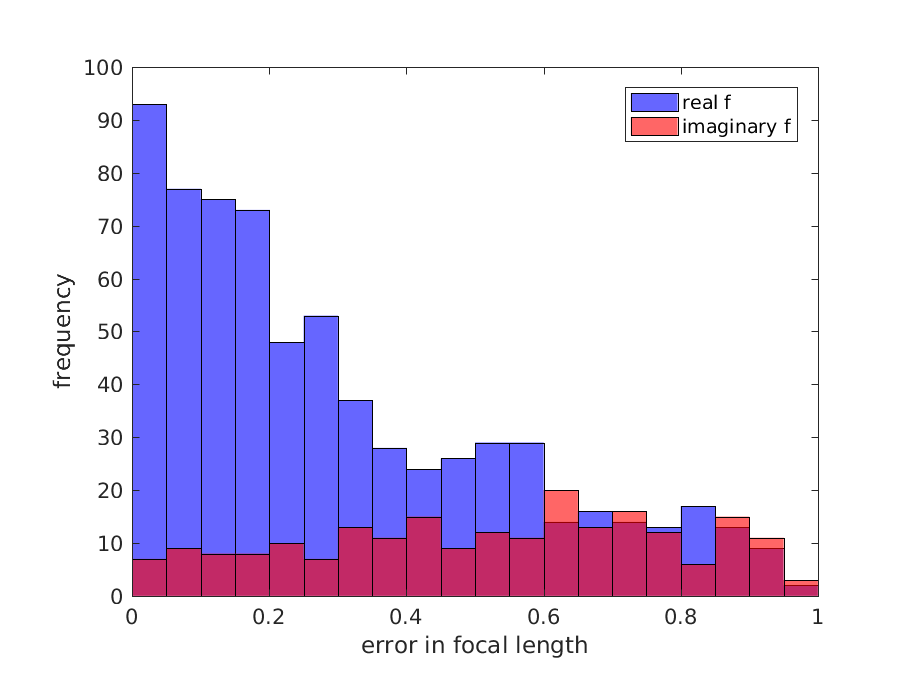
\includegraphics[width=\linewidth]{imaginary_hist.eps}
    \caption[Histogram of errors in the focal length]{The distribution of multiplicative errors (equation \ref{eq:error}) in the focal lengths, produced by 7pt algorithm. Separate distributions are shown for the  case with both real focal lengths (blue) and for the case with at least one imaginary focal length (orange). Red color is shown where the orange is supersimposed over blue. 40 correspondences are used, and level of noise $\sigma$ is equal to 1. }
    \label{imagist}
  \end{center}
\end{figure}


\section{Performance analysis for close to degenerate situations}

In theory, there does not exist a method to recover focal length when the optical axes intersect. With a small amount of noise in the image measurements, however, the configuration no longer is singular. The focal lengths  thus can be computed in almost all practical situations. Nonetheless, we expect pose estimation to deteriorate as the configuration becomes close to singular due to numerical instability. In this section we show the extent of this deterioration.  For the fundamental matrix estimation, we will use the 7pt algorithm, as it apparently performs better than the 8pt algorithm.

\subsection{Intersecting optical axes} 

In this scenario, two non-parallel optical axes are initially in a plane and we lift one camera away from the plane to distance $d$. The optical axes become skew lines. We compare the quality of estimations for different distances $d$ and levels of noise $\sigma$.
In our setup the distance between camera centers is 1 m and the mean distance from the cameras to the scene points is 5 m. 

The Fig.~\ref{interax} shows the distribution of multiplicative errors in the focal length estimates by the 7pt algorithm. The figure shows 4 different levels of noise, and each line represent a distance $d$. We see that for small values of noise, $\sigma \ll 0.1~\text{px}$, the distance between the optical axes significantly affects 7pt algorithm performance.
The performance  deteriorates greatly with decreasing distance between optical axes. For more realistic noise levels, however, the Fig.~\ref{interax} shows that the distance has little impact on the quality of estimation. With 1 pixel noise, the performance is almost the same and axes that are 10 cm or 1 cm apart. A 50 cm transversal configuration, which we assume is not influenced by the degeneration is marginally more suitable for reconstruction. Even for configuration with axes distance zero, the performance is still acceptable (because of the noise in image measurements), with 75\% of estimations being off by a factor of at most 2. 

We suggest this happens because the  noise in image measurements drives the system further away from a degenerate situation. %\TP{delet: The noise effect on camera geometry aprarently has a bias towards moving optical axes further from each other, which reduces the effect of numerical instability.} 


\begin{figure}[h!]
  \begin{center}
    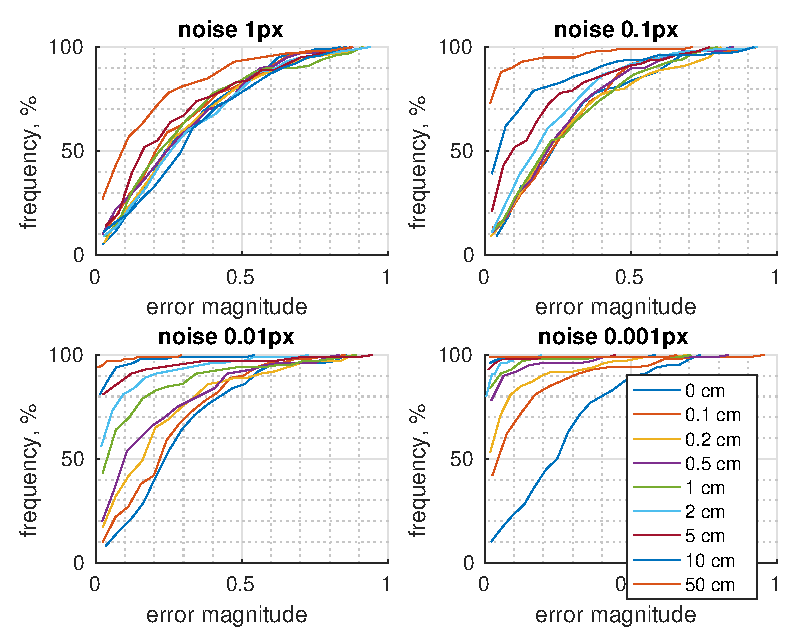
\includegraphics[width=\linewidth]{foc_err_intersecting_axes.eps}
    \caption[Focal length error for intersecting optical axes]{The cumulative distribution of the estimated focal length multiplicative error (equation \ref{eq:error}) for nearly intersecting optical axes. Different lines show different distances between optical axes in centimeters. 7pt algorithm is used}
    \label{interax}
  \end{center}
\end{figure}

\subsection{Parallel optical axes}
An interesting configuration is when the optical axes intersect at a point at infinity, i.e., when they are parallel.

In this scenario, two optical axes are initially parallel and we rotate one axis away from the common plane of the axes by  angle $\alpha$. As we rotate one axis away, it is no longer parallel to the other one. We compare the quality of estimations for different angles $\alpha$ and levels of noise $\sigma$.

Fig.~\ref{parallax} shows the results. We see that the quality of estimation is much worse for  truly parallel axes and small noise in image correspondences does not save the situation. However, the degeneracy almost disappears already when the angle $\alpha$ reaches $0.1^\circ$.


\begin{figure}[h!]
  \begin{center}
    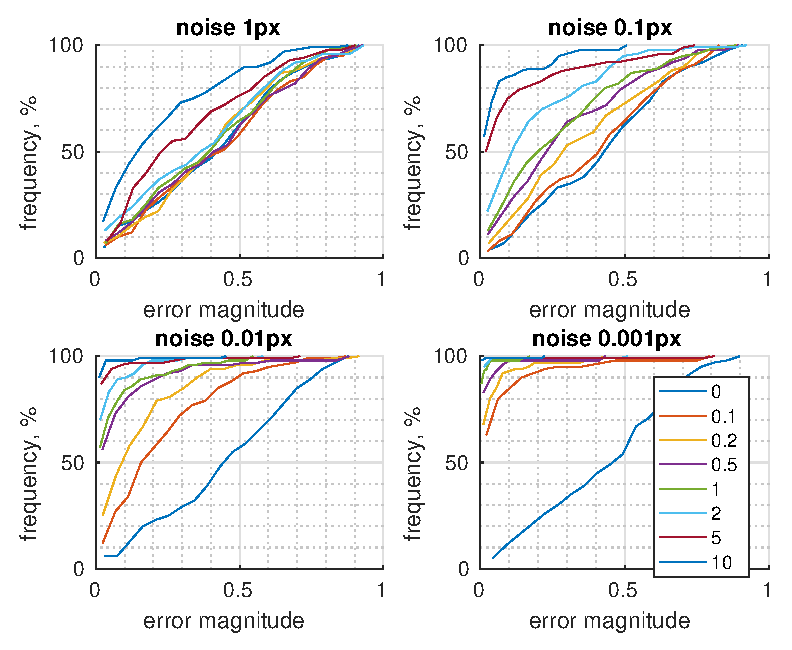
\includegraphics[width=\linewidth]{foc_err_parallel_axes.eps}
    \caption[Focal length error for parallel optical axes]{The cumulative distribution of the estimated focal length multiplicative error (equation \ref{eq:error}) for nearly parallel optical axes. Different lines show different angles between optical axes in degrees. 7pt algorithm is used}
    \label{parallax}
  \end{center}
\end{figure}

\subsection{Conclusions}

We have shown that the 7pt algorithm performs better for most applications. However, interestingly, 8pt algorithm gives less imaginary estimates.

Using more correspondences allows us to make much better results and get imaginary estimates less often. The ratio $r = {f_2}\slash{f_1}$ seems to be more robust than the focal lengths themselves. The ratio is also usable even when the focal lengths are imaginary. 


We confirmed that the imaginary focal lengths are indeed signs of a highly corrupt solution, and the fundamental matrices that decompose into imaginary focal lengths should be discarded.  

Of two types of camera configuration degeneracy, intersecting optical axes do not pose a significant risk for camera reconstruction, especially for real-life noise levels. A configuration with parallel or nearly parallel optical axes, however, is a harder case where more than a half of reconstructions may be off by a factor of two and more.



\chapter{ Algebraic analysis of focal lengths computation}

\label{seq:algeom}

In this section we analyze the methods for computing focal lengths from point correspondences by the algebraic geometry techniques. We show that indeed three and only three fundamental matrices (some possibly complex or of rank 1) can be derived using algebraic geometry. We analyze the degeneracies of the computation. We also show that three different formulae exist for computing focal lengths from a Fundamental matrix. One of these is the Bougnoux formula~\ref{eq:bougnoux1}, and two others weren't known before.
%We show that using the appropriate formula each time, a known degeneracy can be avoided. 

\section{Analysis}
We analyze the set of valid fundamental matrices of  camera pairs  calibrated up to focal lengths using techniques of algebraic geometry. To this end, we use Macaulay2~\cite{Macaulay}, a programming language and also a software pack for algebraic geometry and abstract commutative algebra. Macaulay2 tends to have an intuitive interface for many algebraic operations and, in general, code can be read as easily as mathematical equations. For this reason, instead of mathematical language, we will use in this section Macaulay2 code snippets directly. This helps to make our results reproducible, too.


In algebraic terms, we choose to describe the set of valid $\mathtt{F}$s as a variety in a field of rational numbers $\Q^{11}$ of 11 unknowns, 9 for elements of the fundamental matrix F and 2 for focal lengths $f_1$, $f_2$. We assume that the principal points $\mathbf{p}_1$, $\mathbf{p}_2$ are zero.  

The ideal $Gs$ is the ideal generated by rank \ref{eq:rankF} and trace constraints \ref{eq:trace} and saturated by the ideal $\langle f_1\,f_2 \rangle$. The saturation is desirable, because it can remove large spurious components corresponding to cases when $f_1=0$ or $f_2=0$, which can't happen in any real camera systems.

Below is a snippet of Macaulay2 code explaining the construction of  $Gs$.

\begin{verbatim}
R = QQ[f1,f2,f11,f12,f13,f21,f22,f23,f31,f32,f33, MonomialOrder=>Lex]
F = matrix{{f11,f12,f13},{f21,f22,f23},{f31,f32,f33}}
K1 = matrix{{f1, 0, 0}, {0, f1, 0}, {0, 0, 1}}
K2 = matrix{{f2, 0, 0}, {0, f2, 0}, {0, 0, 1}}
E = transpose(K2)*F*K1 -- Essential matrix
Et = transpose E
G = ideal(det(E)) + minors(1, 2*E*Et*E - trace(E*Et)*E); 
dim G, codim G, degree G
Gs = saturate(G,ideal(f1*f2)); -- det(K1),det(K2) are non-zero
dim Gs, codim Gs, degree Gs -- dimension, codimension and degree
\end{verbatim}

The ideal $Gs$ contains constraints under which a matrix is generically a fundamental matrix. The variety $\textbf{V}(Gs)$ therefore is a variety that contains all valid fundamental matrices. It also contains more matrices, specifically those of rank 0 and 1. Generically, however, we expect a matrix from the variety to be of rank 2. Moreover, when considered in the algebraically closed field $\C$, the variety does contain some complex matrices. In practical situations however, when considering a solver constructed this way, we can just sort out the spurious solutions afterwards as there will be only three solutions in total.

The 7pt algorithm can be regarded as intersecting the variety $\textbf{V}(Gs)$ it with 7 hyperplanes, and it gives us three different solutions. The solutions are actually one-dimensional subspaces, and therefore we would expect the ideal $Gs$ to have dimension 8, which it indeed has.
%\TP{NO. We would expect this to be 8 because the solutions are one-dimensional subspaces since all is homogeneous and we are in a projective space.} and degree 3, but in reality, as constructed, it has dimension of 8 and degree of 58. This is explained by the fact that the variety $\textbf{V}(Gs)$ has an additional component of dimension 8 and degree 58. 
%\OR{there is something wrong with this degree 58 component, but i'd better leave this out altogether}
%Executing 7pt algorithm can be viewed as adding epipolar constraints to the ideal, and later we will see that this component doesn't survive the procedure.

The next snippet shows how to compute algebraic conditions in terms of elements of Fundamental matrix only, by eliminating $f_1,f_2$.

\begin{verbatim}
M = eliminate(Gs,{f1,f2}); 
dim M, codim M, degree M
-- the commands "mingens gb" give a minimal set of generators 
-- for the groebner basis of an ideal 
m = mingens gb M
\end{verbatim}

After executing the above, we see that the ideal $M$ has only one generator - the $\det(\mathtt{F})$ polynomial. This means that the algebraic constraints on the set of fundamental matrices of up to focal lengths calibrated camera pairs are the same as for the fully uncalibrated camera case. It can be deduced that a seven-tuple of corresponding points obtained by completely uncalibrated cameras  can  also  be  explained  by  cameras  with  two  unknown focal lengths when the focal lengths are allowed to attain non-real values.

It also means that only the rank constraint~\ref{eq:rank} is needed to solve the system, and the trace constraint is extraneous. The trace constraint, however, allow us to compute the focal lengths.

\section{Computing focal lengths}
\label{sec:focalformulae}
In the next snippet we show how the Bougnoux formula~\cite{Bougnoux} can be derived with algebraic geometry, given as a polynomial in the entries of F. This is done by eliminating one of the focal lengths from the ideal $Gs$. It turns out that the Gr\"obner basis of the eliminated ideal $s_i$ contains the determinant of $\M{F}$ and additional three polynomials, from which a formula for computing the focal length that wasn't eliminated can be deducted. This means that there exist three algebraically independent constraints on each focal length.

\begin{verbatim}
s2 = mingens gb eliminate(Gs,f1)
s1 = mingens gb eliminate(Gs,f2)
-- Formulae for f1
(m11,c11) = coefficients(s1_1_0,Variables=>{f1}) -- extract coefficients 
(m12,c12) = coefficients(s1_2_0,Variables=>{f1}) -- extract coefficients
(m13,c13) = coefficients(s1_3_0,Variables=>{f1}) -- extract coefficients
-- Formulae for f2
(m21,c21) = coefficients(s2_1_0,Variables=>{f2}) -- extract coefficients 
(m22,c22) = coefficients(s2_2_0,Variables=>{f2}) -- extract coefficients
(m23,c23) = coefficients(s2_3_0,Variables=>{f2}) -- extract coefficients
\end{verbatim}

We see that there exist three formulae for each focal length, for example, 
{\small
%\begin{equation}
\begin{multline}
\label{eq:3}
f^2_2 = - \frac{c23_{0,1}}{c23_{0,0}} =  - \frac{\M{F}_{3,3} (\M{F}_{1,1} \M{F}_{2,3} \M{F}_{3,1}+\M{F}_{1,2} \M{F}_{2,3} \M{F}_{3,2}-\M{F}_{1,3} \M{F}_{2,1} \M{F}_{3,1}-\M{F}_{1,3} \M{F}_{2,2} \M{F}_{3,2})}{\splitdfrac{(\M{F}_{1,1}^2 \M{F}_{1,3} \M{F}_{2,3}-\M{F}_{1,1} \M{F}_{1,3}^2 \M{F}_{2,1}+\M{F}_{1,1} \M{F}_{2,1} \M{F}_{2,3}^2+\M{F}_{1,2}^2 \M{F}_{1,3} \M{F}_{2,3}}{-\M{F}_{1,2} \M{F}_{1,3}^2 \M{F}_{2,2}+\M{F}_{1,2} \M{F}_{2,2} \M{F}_{2,3}^2-\M{F}_{1,3} \M{F}_{2,1}^2 \M{F}_{2,3}-\M{F}_{1,3} \M{F}_{2,2}^2 \M{F}_{2,3})}}.
\end{multline}}
%\end{equation}}
It can be checked that this formula is equivalent to the Bougnoux formula by expressing the latter directly in terms of Fundamental matrix elements. The two other formulae are: 
{\small
\begin{multline}
\label{eq:2}
f^2_2 = - \frac{c22_{0,1}}{c22_{0,0}} =- \dfrac{\M{F}_{3,3} (\M{F}_{1,1} \M{F}_{3,1} \M{F}_{3,3}+\M{F}_{1,2} \M{F}_{3,2} \M{F}_{3,3}-\M{F}_{1,3} \M{F}_{3,1}^2-\M{F}_{1,3} \M{F}_{3,2}^2)}{\splitdfrac{(\M{F}_{1,1}^2 \M{F}_{1,3} \M{F}_{3,3}-\M{F}_{1,1} \M{F}_{1,3}^2 \M{F}_{3,1}+\M{F}_{1,1} \M{F}_{2,1} \M{F}_{2,3} \M{F}_{3,3}+\M{F}_{1,2}^2 \M{F}_{1,3} \M{F}_{3,3}}{-\M{F}_{1,2} \M{F}_{1,3}^2 \M{F}_{3,2}+\M{F}_{1,2} \M{F}_{2,2} \M{F}_{2,3} \M{F}_{3,3}-\M{F}_{1,3} \M{F}_{2,1} \M{F}_{2,3} \M{F}_{3,1}-\M{F}_{1,3} \M{F}_{2,2} \M{F}_{2,3} \M{F}_{3,2})}}.
\end{multline}}
{\small
\begin{multline}
\label{eq:1}
f^2_2 = - \frac{c21_{0,1}}{c21_{0,0}}  =-\dfrac{\M{F}_{3,3} (\M{F}_{2,1} \M{F}_{3,1} \M{F}_{3,3}+\M{F}_{2,2} \M{F}_{3,2} \M{F}_{3,3}-\M{F}_{2,3} \M{F}_{3,1}^2-\M{F}_{2,3} \M{F}_{3,2}^2)}{\splitdfrac{(\M{F}_{1,1} \M{F}_{1,3} \M{F}_{2,1} \M{F}_{3,3}-\M{F}_{1,1} \M{F}_{1,3} \M{F}_{2,3} \M{F}_{3,1}+\M{F}_{2,1}^2 \M{F}_{2,3} \M{F}_{3,3}-\M{F}_{2,1} \M{F}_{2,3}^2 \M{F}_{3,1}}{+\M{F}_{1,2} \M{F}_{1,3} \M{F}_{2,2} \M{F}_{3,3}-\M{F}_{1,2} \M{F}_{1,3} \M{F}_{2,3} \M{F}_{3,2}+\M{F}_{2,2}^2 \M{F}_{2,3} \M{F}_{3,3}-\M{F}_{2,2} \M{F}_{2,3}^2 f_{3,2})}}.
\end{multline}}

The formulae for the other focal length $f_1$ may be obtained by transposing the fundamental matrix. The undertaken analysis of the formulae has shown that generically they differ little in terms of stability and quality of estimations. However, as the denominators of the formulae are different, each of them has its own degeneracies, where another one may succeed instead.
We proceed to give examples of such situations.

It can be shown by substitution that the Bougnoux formula vanishes whenever either first or second column of $\mathtt{F}$ is the zero vector. Of the formulae we found, however, the third formula (Eq.~\ref{eq:1}) does not necessarily vanish when the first column of $\mathtt{F}$ is zero, and the second formula (Eq.~\ref{eq:2}) does not necessarily vanish when the second column is zero. When the third column is zero, all the formulae either vanish or become $p(\M{F})\,f_2^2=0$. The focal lengths cannot be reconstructed in this case per lemma~\ref{interlemma}, as $\mathtt{F}_{3,3}=0$. 

\begin{exmp}
\label{ex:tilt}
The pair of cameras $\M{P}_1$, $\M{P}_2$ both have their optical axes almost perpendicular to the baseline (tilted by an angle of $\pi \slash 10$) and experience the degeneration where the plane defined by the baseline and the optical axis of one camera is perpendicular to the plane defined by the baseline and optical axis of the other camera~\cite{HartZiss}. The calibration matrices are identity matrices. More precisely, the fundamental matrix of the pair is:

\begin{align*}
    & R^{tilt} = \mat{ccc}{\cos (\pi \slash 10) & 0 & \sin (\pi \slash 10) \\ 0 & 1 & 0 \\ -\sin (\pi \slash 10) & 0 & \cos (\pi \slash 10)} \\
    & \M{F}= \M{R} * \cross{t} = R^{tilt}    
    \mat{ccc}{1 & 0 & 0 \\ 0 & 0 & -1 \\ 0 & 1 & 0}
    R^{tilt}
    \mat{ccc}{0 & 0 & 0 \\ 0 & 0 & -1 \\ 0 & 1 & 0} 
    \approx \mat{ccc}{0 & 0.3 & 0.3 \\ 0 & 0.9 & 0 \\ 0 & 0.1 & 0.9 }
\end{align*}


By substitution, the first and second (Eqs.~\ref{eq:2},~\ref{eq:3}) vanish on this example,, i.e., assume the form $  0 \; f_2^2 = 0 $, but the third formula (Eq.~\ref{eq:1}) successfully gives a correct focal length estimate.

\end{exmp}

The example~\ref{ex:tilt} shows that there among all configurations known to be degenerate for the Bougnoux formula, there exist some that can be successfully solved by using the correct formula of the existing three. We see that specifically the degeneration  when the plane defined by the baseline and the optical axis of one camera is perpendicular to the plane defined by the baseline and optical axis of the other camera can be, at least in some cases, solved. We also see that in the example~\ref{ex:tilt} the configuration corresponds to a fundamental matrix which has the first column equal to zero vector.
%We also conjecture that this happens when first or second column is zero occurs


Note that there still remains a degeneracy when each of the three denominators vanishes. When this happens, the focal lengths cannot be reconstructed from the matrix $\mathtt{F}$, as there are no constraints on them (they can have any value). The next example shows when this degeneracy might occur.

\begin{exmp}
\label{ex:fail}
The pair of cameras $\M{P}_1$, $\M{P}_2$ are similar as in the example~\ref{ex:tilt}, but without tilt, i.e., they both have their optical axes perpendicular to the baseline. They also experience the degeneration where the plane defined by the baseline and the optical axis of one camera is perpendicular to the plane defined by the baseline and optical axis of the other camera. The calibration matrices are identity matrices. More precisely, the fundamental matrix of the pair is:

\begin{equation*}
    \M{F}= \M{R} * \cross{t} = \mat{ccc}{1 & 0 & 0 \\ 0 & 0 & -1 \\ 0 & 1 & 0}  \mat{ccc}{0 & 0 & 0 \\ 0 & 0 & -1 \\ 0 & 1 & 0} = \mat{ccc}{0 & 0 & 0 \\ 0 & -1 & 0 \\ 0 & 0 & -1}
\end{equation*}

By substitution, all three formulae (Eqs.~\ref{eq:1}~\ref{eq:2},~\ref{eq:3}) vanish on this example, i.e., assume the form $  0 \; f_2^2 = 0 $

\end{exmp}


Based on the examples~\ref{ex:tilt},~\ref{ex:fail} we \textit{conjecture} that the remaining degeneracy is the case when the both camera have their optical axes perpendicular to the baseline, and also experience the degeneration where the plane defined by the baseline and the optical axis of one camera is perpendicular to the plane defined by the baseline and optical axis of the other camera. In this case all three formulae should fail.

\section{The ratio formula}
We present a formula to compute directly the ratio $r = f_2 \slash f_1$. Note that unlike focal length formulae, there can be only one algebraically independent formula for computing the ratio.

% tex.stackexchange.com/questions/180917/breaking-the-equation-inside-a-fraction

{\tiny
\begin{equation}
r = \frac{f_2}{f_1} =  
\dfrac{\splitdfrac{\splitdfrac{\M{F}_{1,1}^2 \M{F}_{3,1}^2 \M{F}_{3,3}+2 \M{F}_{1,1} \M{F}_{1,2} \M{F}_{3,1} \M{F}_{3,2} \M{F}_{3,3}-\M{F}_{1,1} \M{F}_{1,3} \M{F}_{3,1}^3-\M{F}_{1,1} \M{F}_{1,3} \M{F}_{3,1} \M{F}_{3,2}^2}{+\M{F}_{1,2}^2 \M{F}_{3,2}^2 \M{F}_{3,3}-\M{F}_{1,2} \M{F}_{1,3} \M{F}_{3,1}^2 \M{F}_{3,2}-\M{F}_{1,2} \M{F}_{1,3} \M{F}_{3,2}^3+\M{F}_{2,1}^2 \M{F}_{3,1}^2 \M{F}_{3,3}+2 \M{F}_{2,1} \M{F}_{2,2} \M{F}_{3,1} \M{F}_{3,2} \M{F}_{3,3}}}{-\M{F}_{2,1} \M{F}_{2,3} \M{F}_{3,1}^3-\M{F}_{2,1} \M{F}_{2,3} \M{F}_{3,1} \M{F}_{3,2}^2+\M{F}_{2,2}^2 \M{F}_{3,2}^2 \M{F}_{3,3}-\M{F}_{2,2} \M{F}_{2,3} \M{F}_{3,1}^2 \M{F}_{3,2}-\M{F}_{2,2} \M{F}_{2,3} \M{F}_{3,2}^3}}{\splitdfrac{\splitdfrac{\M{F}_{1,1}^2 \M{F}_{1,3}^2 \M{F}_{3,3}-\M{F}_{1,1} \M{F}_{1,3}^3 \M{F}_{3,1}+2 \M{F}_{1,1} \M{F}_{1,3} \M{F}_{2,1} \M{F}_{2,3} \M{F}_{3,3}-\M{F}_{1,1} \M{F}_{1,3} \M{F}_{2,3}^2 \M{F}_{3,1}}{+\M{F}_{1,2}^2 \M{F}_{1,3}^2 \M{F}_{3,3}-\M{F}_{1,2} \M{F}_{1,3}^3 \M{F}_{3,2}+2 \M{F}_{1,2} \M{F}_{1,3} \M{F}_{2,2} \M{F}_{2,3} \M{F}_{3,3}-\M{F}_{1,2} \M{F}_{1,3} \M{F}_{2,3}^2 \M{F}_{3,2}}}{-\M{F}_{1,3}^2 \M{F}_{2,1} \M{F}_{2,3} \M{F}_{3,1}-\M{F}_{1,3}^2 \M{F}_{2,2} \M{F}_{2,3} \M{F}_{3,2}+\M{F}_{2,1}^2 \M{F}_{2,3}^2 \M{F}_{3,3}-\M{F}_{2,1} \M{F}_{2,3}^3 \M{F}_{3,1}+\M{F}_{2,2}^2 \M{F}_{2,3}^2 \M{F}_{3,3}-\M{F}_{2,2} \M{F}_{2,3}^3 \M{F}_{3,2}}}
\end{equation}
}

Computing the ratio directly from $\mathtt{F}$ can offer  greater speed and more stability than computing it from the focal lengths. Indeed, we observed that for close to degenerate situations, the formula,  although marginally, is a better estimator. 

\section{Computing Fundamental matrices}

We show in detail how the 7pt solver works from the viewpoint of algebraic geometry.

% In the next snippet of code we simulate a random scene\footnote{The simulated points may occur in a singular configuration. If this happens, rank of the matrix $\mathtt{A}$  will not be 7, and there will be an infinite number of possible matrices $\mathtt{F}$. This, however, can almost never happen.}

% \begin{verbatim}
% fl1=1500
% fl2=2000
% K1 = matrix{{fl1,0,0},{0,fl1,0},{0,0,1}}
% K2 = matrix{{fl2,0,0},{0,fl2,0},{0,0,1}}
% R2 = matrix{{0,1,0},{-3/5,0,4/5},{4/5,0,3/5}} * matrix{{1,0,0},{0,3/5,-4/5},{0,4/5,3/5}} ** 
% R1 = id_(R^3)
% points=7
% X  = matrix(fillMatrix(mutableMatrix(QQ,4,points)))
% X =  mutableMatrix for i from 0 to points-1 list (1/X_i_3)*(X_i)
% for i from 0 to points-1 do X_(2,i)=X_(2,i)+3
% X = matrix X
% t1 = transpose matrix{{0,0,0}}
% t2 = transpose matrix{{-1,-1,-1}}
% P1=K1*(R1| -R1*t1)
% P2=K2*(R2| -R2*t2)

% u1=P1*X
% u2=P2*X

% B = transpose matrix for i from 0 to points-1 list u1_i ** u2_i 

% \end{verbatim}


We first simulate a random set of correspondences. We skip this code for brevity and assume that the matrix $\mathtt{B}$ is a matrix from the 7pt algorithm (algorithm \ref{7pt}), i.e., the matrix, the right null space of which is the linear space of all (vectorized) matrices satisfying 7 certain epipolar constraints~\ref{eq:epipolar}. 

In the next snippet we show detailed analysis of the computation results. The variety $\textbf{V}(GBs)$ is the variety of all possible focal lengths that explain the simulated correspondences.

\begin{verbatim}
m = transpose matrix {{f11,f12,f13,f21,f22,f23,f31,f32,f33}}
rank B
eB = B*m
IB = minors(1,eB)
GBs = Gs + IB
gGBS=mingens gb GBs
dim GBs, codim GBs, degree GBs
pGBS = minimalPrimes GBs
\end{verbatim}

Ideal $IB$ contains the epipolar constraints. By adding together the ideals $Gs$ and $IB$ we combine the constraints and obtain an ideal that corresponds to a variety of solutions of the 7pt solver for our correspondences.

Variety $\textbf{V}(GBs)$ can consist of either 5 or 13 components, one of dimension 2, and the rest of dimension 0. We will show the significance of this fact and what are these components corresponding to.

We provide an example of what the minimal primes (ideals, corresponding to component varieties) may look like. 

\begin{exmp}
The \textit{minimal primes} of an ideal containing seven epipolar constraints and the rank constraint. The actual minimal primes are 6 ideals, which correspond to 5 component varieties over $\Q$. One of the prime ideals does not correspond to any variety over $\Q$, but would decompose into 8 point varieties over $\C$. We exclude this ideal from the example for the sake of brevity. The remaining 5 ideals are as follows:
\begin{enumerate}
    \item   $\langle\M{F}_{3,3}$, $\M{F}_{3,2}$, $\M{F}_{3,1}$, $\M{F}_{2,3}$, $\M{F}_{2,2}$, $\M{F}_{2,1}$, $\M{F}_{1,3}$, $\M{F}_{1,2}$, $\M{F}_{1,1}\rangle$
    \item $\langle16000 \M{F}_{3,2} + 31 \M{F}_{3,3}$, $3200 \M{F}_{3,1} + 3 \M{F}_{3,3}$, $12000 \M{F}_{2,3} + 11 \M{F}_{3,3}$, $8000000 \M{F}_{2,2} - 9 \M{F}_{3,3}$, $1200000 \M{F}_{2,1} + \M{F}_{3,3}$, $4000 \M{F}_{1,3} - \M{F}_{3,3}$, $       6000000 \M{F}_{1,2} - \M{F}_{3,3}$, $4800000 \M{F}_{1,1} - 7 \M{F}_{3,3}$, $f_2 + 1500$, $f_1 - 2000\rangle$ 
    \item  $\langle16000 \M{F}_{3,2} + 31 \M{F}_{3,3}$, $3200 \M{F}_{3,1} + 3 \M{F}_{3,3}$, $12000 \M{F}_{2,3} + 11 \M{F}_{3,3}$, $8000000 \M{F}_{2,2} - 9 \M{F}_{3,3}$, $1200000 \M{F}_{2,1} + \M{F}_{3,3}$, $4000 \M{F}_{1,3} - \M{F}_{3,3}$, $6000000 \M{F}_{1,2} - \M{F}_{3,3}$, $4800000 \M{F}_{1,1} - 7 \M{F}_{3,3}$, $f_2 + 1500$, $f_1 +        2000\rangle$
    \item $\langle16000 \M{F}_{3,2} + 31 \M{F}_{3,3}$, $3200 \M{F}_{3,1} + 3 \M{F}_{3,3}$, $12000 \M{F}_{2,3} + 11 \M{F}_{3,3}$, $8000000 \M{F}_{2,2} - 9 \M{F}_{3,3}$, $1200000 \M{F}_{2,1} + \M{F}_{3,3}$, $4000 \M{F}_{1,3} - \M{F}_{3,3}$, $6000000 \M{F}_{1,2} - \M{F}_{3,3}$, $4800000 \M{F}_{1,1} - 7 \M{F}_{3,3}$, $f_2 -        1500$, $f_1 + 2000\rangle$
    \item $\langle16000 \M{F}_{3,2} + 31 \M{F}_{3,3}$, $3200 \M{F}_{3,1} + 3 \M{F}_{3,3}$, $12000 \M{F}_{2,3} + 11 \M{F}_{3,3}$, $8000000 \M{F}_{2,2} - 9 \M{F}_{3,3}$, $1200000 \M{F}_{2,1} + \M{F}_{3,3}$, $4000 \M{F}_{1,3} - \M{F}_{3,3}$, $6000000 \M{F}_{1,2} - \M{F}_{3,3}$, $4800000 \M{F}_{1,1} - 7        \M{F}_{3,3}$, $f_2 - 1500$, $f_1 - 2000\rangle$
\end{enumerate}
\end{exmp}


The first ideal corresponds to the component of dimension 2. It represents the degenerate situation when  the matrix $\M{F}$ is the zero matrix. The ideal also does not contain any polynomial in $f_1$ or $f_2$, so neither of focal lengths can be determined as there are no constraints on them. Because of this, the component has dimension 2, its two degrees of freedom are $f_1$ and $f_2$.

% I might be wrong writing this one
% The first component contains the polynomials $f_1$ and $f_2$, which means that  it corresponds to a degenerate case when $f_1=0, f_2=0$. Technically, such a fundamental matrix satisfies all constraints and is an example of a matrix having rank less than two (see the discussion in section \ref{seq:failure}). This case could be avoided by using  unknowns $w_1=\frac{1}{f_1}, w_2=\frac{1}{f_2}$. \TP{I tried it and there is a case f(F,w1,w2)=0. Which still needs to be analyzed.} \OR{what is f?}\TP{f stands here for a polynomial, its really a bit confusing}

The 12 (or 4) other components are of dimension 0 are point varieties (all  unknowns are determined there). They  can be divided into 3 groups (or 1 group), which correspond(s) to 3 different Fundamental matrices (a single matrix). Each group includes 4 point varieties in form $f_1 = \pm  C_1, f_2 \pm C_2$ where $C_1, C_2$ are constants. The reason for this is that the focal length actually only enters the Bougnoux formula, as well as formulae we derived (Eqs.~\ref{eq:1},~\ref{eq:2},~\ref{eq:3}) in the second degree, so it is impossible to determine it's sign\footnote{Of course for any practical application the situation is unambiguous, as the positive sign should always be chosen.}.

We see that each group corresponds to one of the three fundamental matrices as returned by 7pt algorithm. Sometimes, however, two of them would be complex. In this case we will get only one group, as our code considers varieties over real numbers. This explains why sometimes we can get only 4 components with nonzero $f_1, f_2$ instead of 12.


\section{Conclusions}

We have shown how Bougnoux formula and 7pt algorithm work in terms of algebraic geometry. We have derived 2 new formulae for computing focal lengths from fundamental matrix, and a formula for computing ratio $r = f_2 \slash f_1$. No more algebraically independent formulae can be derived for this problem.
We have shown that a known degeneracy \cite{HartZiss} can be partially avoided by using the right focal length formula of the three. The degeneracy reduces to the case when all three formulae fail.

We  confirmed that three and only three fundamental matrices can explain 7 correspondences. 
We have shown that the trace constraint is redundant while solving camera relative pose with two unknown focal lengths.


\chapter{Improvements}


\label{seq:thenew}

Using the analysis carried out in the previous chapters, we suggest  improvements to the existing methods of focal length computing.

\section{f-Ratio}
We present and analyze the performance of a new algorithm, called f-Ratio, for robust focal lengths computation. The algorithm uses the premise that the ratio of focal lengths is more robust to achieve superior accuracy. The algorithm serves as a further proof that explicitly using the ratio of the focal lengths may by beneficial for the performance.

\subsection{Algorithm}

The idea of the algorithm is to use a new solver that would compute $\mathtt{F}$ from 6 correspondences given the ratio $r=f_2 \slash f_1$. We create such a solver using the automatic generator~\cite{generator}. The solver uses the Demazure polynomials, i.e.\ the rank and the constraints~\ref{eq:rank},~\ref{eq:trace} in terms of elements of the matrix $\mathtt{F}$, $f_1$, and $r$. 

 A solver assuming fixed focal length $f_1=f_2$ could be used instead, for example that of Torii et el.~\cite{Aki6pt}, by first rescaling \[\V{x}_2^{r}= \mat{ccc}{r & 0 & 0 \\ 0 & r & 0 \\ 0 & 0 & 1} \V{x}_2.\] The output of such solver would be $f_1$ and $\mathtt{F}$. We can compute $f_2$ as $f_1  r$.  

Both solvers give same results up to machine precision. Both solvers also yield 15 (possibly non-real) solutions. 

\begin{algorithm}[H]
\SetAlgoNoLine
\LinesNotNumbered
\KwData{A list of 7 right image points $\V{x}_1$ and a list of the corresponding left image points $\V{x}_2$, lists of remaining tentative correspondences $\V{x}_1^{test}, \V{x}_2^{test}$, 6pt solver $solve6pt$}
\KwResult{Fundamental matrix $F$}
 \Begin
    {Estimate $\M{F}_0$ from all correspondences\;
    
    Estimate $r=f_2 \slash f_1$ from $\M{F}_0$ \;
    
    \ForEach{6-tuple $\V{x}_1^6$ of points drawn from $\V{x}_1$} 
        {
        $\V{x}_2^6 \leftarrow$ corresponding points to $\V{x}_1^6$ from $\V{x}_2$ \;
        $\M{F}s_i \leftarrow solve6pt(\V{x}_1^6,\V{x}_2^6,r)$\;
        $\M{F}_i \leftarrow$ the matrix from $ \M{F}s_i$ which best explains $\V{x}_1^{test}, \V{x}_2^{test}$,
        }
        
    \Return{$F_i$ which best explains $\V{x}_1^{test}, \V{x}_2^{test}$}
    }
 \caption{f-Ratio}
 \label{f-Ratio}
\end{algorithm}

The solver needs to compute and test 7 $\times$ 15 fundamental matrices\footnote{At most. The 6pt solver usually gives from 9 to 14 real solution, but the maximal possible number is 15. }, which still may be bearable time for a RANSAC-based method. 

One may construct a version of the algorithm which works with all the available points, however,  in such an algorithm one would need to test a combinatorially growing number of matrices.
%\footnote{At most. The 6pt solver usually gives from 9 to 14 real solution, but the maximal possible number is 15. }
%, the amount of computation needed is much bigger. 

\subsection{Performance}

We assess the performance of the algorithm in a similar manner as in the previous analysis. Fig.~\ref{fratio_nonoise} a comparison our f-Ratio method and the baseline 7pt algorithm. 

\begin{figure}[h!]
  \begin{center}
    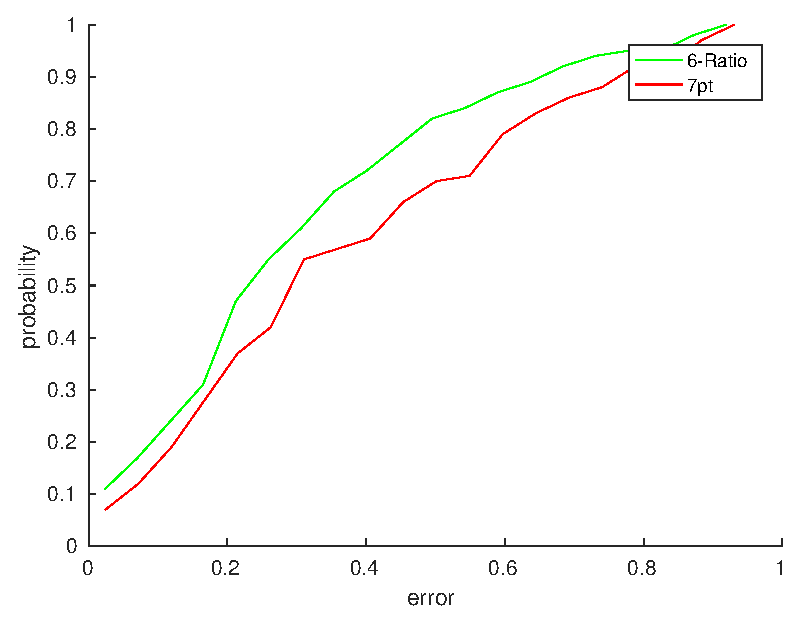
\includegraphics[width=\linewidth]{ratio6_nonoise.eps}
    \caption[Performance of f-Ratio]{A comparison of 6-Ratio against the baseline. The cumulative distribution of the  multiplicative error (equation \ref{eq:error})  in the focal  length  estimates is shown.}
    \label{fratio_nonoise}
  \end{center}
\end{figure}

In the next experiment, Fig.~\ref{fratio_10noise} we add an additional amount of noise ($\sigma=10$ pixels) to one of the points. This demonstrates that our method can cope with outliers even better than the standard RANSAC algorithm.

\begin{figure}[h!]
  \begin{center}
    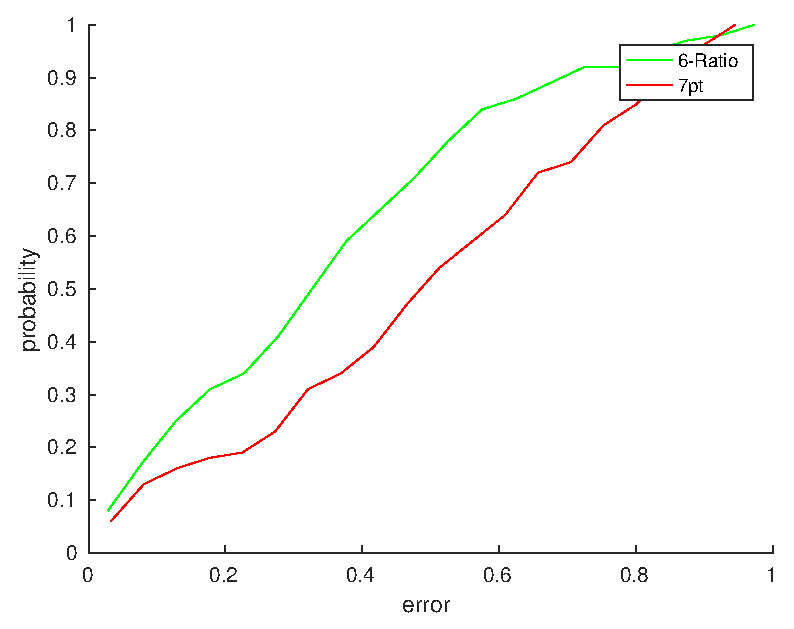
\includegraphics[width=\linewidth]{ratio6_10noise.eps}
    \caption[Performance of f-Ratio with one outlier]{A comparison of 6-Ratio against the baseline in presence of outliers. The cumulative distribution of the  multiplicative error (equation \ref{eq:error})  in the focal  length  estimates is shown. }
    \label{fratio_10noise}
  \end{center}
\end{figure}

The results show that it is possible to reconstruct  scenes better with f-Ratio than with 7pt algorithm. The algorithm  \ref{f-Ratio} successfully demonstrates that explicitly using estimated ratio of focal lengths
%over the focal lengths themselves
may improve the accuracy of the estimation.

\section{Prior focal length}

Hartley~\cite{HartleyPriors} describes an iterative algorithm for computing focal lengths from point correspondences, which incorporates prior information about focal lengths and principal points. The algorithm uses a Levenberg-Marquardt optimization. In this section we describe an improvement to his algorithm. Using computed focal length ratio $r=f_2 \slash f_1$, we are able to get better focal lengths estimates.

\subsection{Original Hartley's algorithm}

Original Hartley's algorithm optimizes a certain cost function given the weights $w_i$, point correspondences $\mathtt{x}_1$, $\mathtt{x}_2$, prior focal length  $\bar{f}_1$, $\bar{f}_2$, minimal focal length $f_{min}$ and prior principal points $\bar{\mathbf{p}}_1$, $\bar{\mathbf{p}}_2$. We give this cost function as algorithm \ref{alg:hart_cost}. 


Note that the focal lengths are not in the list of the parameters to this cost function, as they are determined by the fundamental matrix and principal points.

\begin{algorithm}
\SetAlgoLined 
\LinesNotNumbered
 \KwData{Fundamental matrix $\mathtt{F}$, principal points $\mathbf{p}_1$, $\mathbf{p}_2$.}
 \KwResult{Vector of costs (errors) $\mathbf{C}$}
 \Begin
    {From $\mathtt{F}$, $\mathbf{p}_1$, $\mathbf{p}_2$ compute $f_1$, $f_2$\;
    
    $C_\mathtt{F} \leftarrow$ Sampson error of the matrix $\mathtt{F}$ on the points $\mathtt{x}_1$, $\mathtt{x}_2$\;
    
    
    $C_f \leftarrow w_1^2(f_1^2-\bar{f}_1^2)^2 + w_2^2(f_2^2-\bar{f}_2^2)^2  + w_d^2(f_1^2-f_2^2)^2 + w_{z1}^2(f_{min}^2 - f_1^2)^2 + w_{z2}^2(f_{min}^2-f_2^2)^2 $\;
    
    $C_\mathbf{p} \leftarrow w_p^2 \norm{\mathbf{p}_1-\bar{\mathbf{p}}_1}^2 + w_p^2 \norm{\mathbf{p}_2-\bar{\mathbf{p}}_2}$\;
    
    \Return{Costs $C_\mathtt{F}$, $C_\mathbf{p}$, $C_f$\;}}
 \caption{The cost function of Hartley~\cite{HartleyPriors}}
 \label{alg:hart_cost}
\end{algorithm}


The cost function of focal lengths $C_f$ incorporates a few interesting ideas besides using prior knowledge in first two terms. Its third term drives the focal lengths to the same value, which probably reflects the fact that most real cameras have similar focal lengths from a relatively small (compared to infinity) range. Also using such a term, the method should perform accurately even if the cameras used were indeed the same camera. The fourth and the fifth terms serve two purposes. Firstly, they prevent the squared focal lengths $f_1^2$, $f_2^2$ from becoming negative, which addresses the problem of imaginary focal lengths estimates. Secondly, these terms also prevent focal lengths from converging to zero. % Can this really happen when using Sampson error instead of x2 F x1 error?

Hartley suggests initializing the optimization with a technique he calls calibrated reconstruction, which is described as algorithm~\ref{alg:calrec}. The algorithm takes point correspondences and prior information about camera calibration, and returns a matrix which is consistent with priors. Hartley also claims that the returned matrix has small Sampson error on the point correspondences.

\begin{algorithm}
\SetAlgoLined 
\LinesNotNumbered
 \KwData{Point correspondences $\V{x}_1$, $\V{x}_2$, prior focal lengths $\bar{f}_1$, $\bar{f}_2$,prior principal points $\bar{\V{p}}_1$,$\bar{\V{p}}_2$.}
 \KwResult{Fundamental matrix $\M{F'}$}
 \Begin
    {Compute a fundamental matrix $\M{F}$ from point correspondences $\V{x}_1$, $\V{x}_2$ using the 7pt algorithm\;
    
    Create the prior calibration matrices $\bar{\M{K}}_1$, $\bar{\M{K}}_2$ from the $\bar{f}_1$, $\bar{f}_2$, $\bar{\V{p}}_1$,$\bar{\V{p}}_2$\; 
    
    Create an estimate of the essential matrix $\bar{\M{E}} = \bar{\M{K}}_2^T \M{F} \bar{\M{K}}_1$\;
    
    Compute $(\M{U}, \M{S}, \M{V}) = \text{svd} (\bar{\M{E}})$\;
    
    Take the two biggest singular values $s_1$, $s_2$
    Create an essential matrix $\M{E} = \M{U} \; \diag(\mat{ccc}{s_1 & s_2 & 0}) \; \M{V}$\;
    
    Create  a fundamental matrix which is consistent with the priors $\M{F}' =  \bar{\M{K}}_2^{-\T} \M{E} \bar{\M{K}}_1^{-1}$\;

    \Return{$\M{F}'$\;}
    }
 \caption{Calibrated reconstruction~\cite{HartleyPriors}}
 \label{alg:calrec}
\end{algorithm}


\subsection{Using ratio}

We introduce a modification based on use of estimated ratio of focal lengths $r= f_2\slash f_1$.  Given the correspondences, we use 7pt algorithm \ref{7pt} and the Bougnoux formula to estimate the ratio. We include the estimated ratio in cost function on $f$ from the function \ref{alg:hart_cost}: \[ C_f = w_1^2(f_1^2-\bar{f}_1^2)^2 + w_2^2(f_2^2-\bar{f}_2^2)^2  + w_d^2((r f_1)^2-f_2^2)^2 + w_{z1}^2(f_{min}^2 - f_1^2)^2 + w_{z2}^2(f_{min}^2-f_2^2)^2. \]

We show that such enhanced solver produces better focal length estimates. The graph \ref{hartley_ratio} shows the experiment with 100 runs of each solver.

\begin{figure}
  \begin{center}
    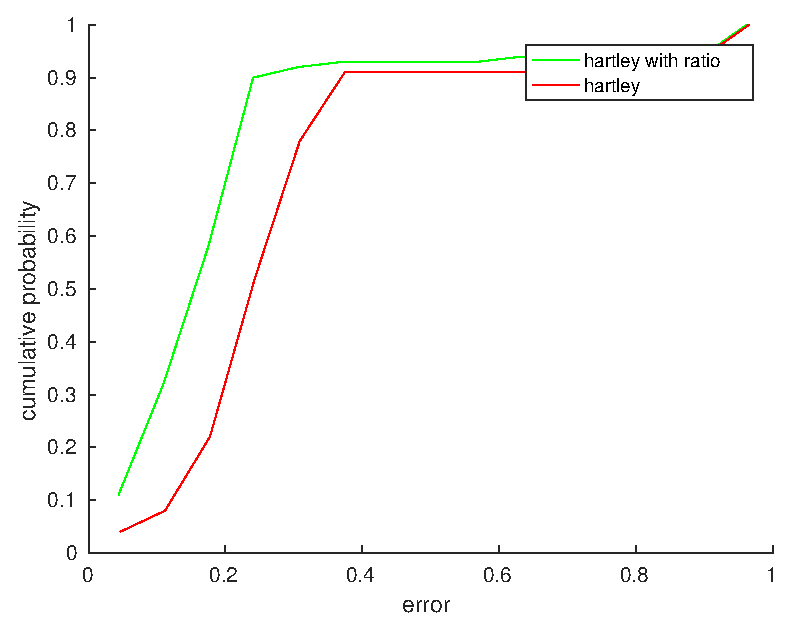
\includegraphics[width=\linewidth]{hartley_ratio_error.eps}
    \caption[Performance of Hartley solver with or without using ratio]{A comparsion of the Hartley algorithm~\cite{HartleyPriors} against our modified version which explicitly uses the ratio of the focal lengths $r = f_2 \slash f_1$ .  The cumulative distribution  of the  multiplicative error (equation \ref{eq:error})  in the focal  length  estimates.  The ground truth focal lengths were $(3,4)$. The prior focal lengths  were  drawn from an uniform distribution between $(3,4)$ and $(4.5, 5.5)$. The ground truth principal points were zero, and the prior principal points were $(0.1, 0.1)$. The number of correspondences used was 40, and the level of noise $\sigma$ was equal to 1. The weights on principal point priors were 10 times smaller than weights on focal lengths priors. }
    \label{hartley_ratio}
  \end{center}
\end{figure}

\subsection{Comparison of focal length computing methods}

We summarize the performance of several methods for estimating the focal lengths from the point correspondences. Besides previously mentioned, we use a method similar to the one from~\cite{Chandraker}. The method derived in the work is described as the algorithm~\ref{alg:Chandraker}

\begin{algorithm}[H]
\SetAlgoLined 
\LinesNotNumbered
 \KwData{Weights $w_i$, point correspondences $\mathtt{x}_1$, $\mathtt{x}_2$, prior focal length  $\bar{f}_1$, $\bar{f}_2$, prior principal points $\bar{\mathbf{p}}_1$, $\bar{\mathbf{p}}_2$.}
 \KwResult{Vector of costs (errors) $\mathbf{C}$}
 \Begin
    {Estimate the fundamental matrix $\mathtt{F}$ using the 7pt algorithm\;
    
    Define $p_1(f_1, f_2, \V{p}_1,\V{p}_2), p_2(f_1, f_2, \V{p}_1,\V{p}_2), p_3(f_1, f_2, \V{p}_1,\V{p}_2)$ as Kruppa equations~\cite{HartZiss}, rewritten as polynomials (see the paper~\cite{Chandraker})\;
    
    Minimize the following cost function:
    \begin{align*}
    %\label{eq:Chandraker}
    & f_1^*, f_2^*, \V{p}_1^*,\V{p}_2^* = & \\ = & \min_{f_1, f_2, \V{p}_1, \V{p}_2, \lambda_1, \lambda_2, \lambda_3} & w_1^2 (f_1 - \bar{f}_1)^2 + w_2^2 (f_2 - \bar{f}_2)^2  + w_p^2 \norm{\mathbf{p}_1-\bar{\mathbf{p}}_1}^2 + w_p^2 \norm{\mathbf{p}_2-\bar{\mathbf{p}}_2} \\ & \text{such that } & \lambda_1 p_1(f_1, f_2, \V{p}_1,\V{p}_2)+ \lambda_2 p_2(f_1, f_2, \V{p}_1,\V{p}_2) + \lambda_3 p_3(f_1, f_2, \V{p}_1,\V{p}_2)
    \end{align*}

    \Return{focal lengths $f_1, f_2$, principal points $\V{p}_1,\V{p}_2$\;}
    }
 \caption{The algorithm of Chandraker~\cite{Chandraker}}
 \label{alg:Chandraker}
\end{algorithm}

Note that the algorithm~\ref{alg:Chandraker}, contrary to the algorithm~\ref{alg:hart_cost} of Hartley, does not  change the fundamental matrix during the optimization. Instead, it computes the fundamental matrix beforehand, and the optimization finds a suitable combination of principal points and focal lengths that would be consistent with the fundamental matrix..

We use an optimization procedure obtained in private conversation to do the optimization in the last step of the algorithm~\ref{alg:Chandraker}.

The figures~\ref{opt_comp_f1}, \ref{opt_comp_f2} show the distribution of focal length as computed by different methods against different levels of noise in prior focal lengths. The distribution for each case is depicted using MATLAB function boxplot which shows 25$\%$ to 75$\%$ quantile values as boxes with a horizontal line for median. The crosses show data beyond 1.5 times the interquartile range. We use high level of noise ($\sigma$ = 4 pixels) to show that the regularization by priors allows us to handle bigger amount of noise. For smaller amounts noise  the difference between the Bougnoux formula and prior methods is not as pronounced.

We can observe in the figures~\ref{opt_comp_f1}, \ref{opt_comp_f2} that different methods behave inherently in a different way. The bougnoux formula has the biggest standard deviation of all, generally is noisy and gives a lot of outliers. The formula is also much less biased, and, of course, is independent of the given prior. The method of Hartley, because of the chosen cost function, tends to drive the focal lengths close to each other. Thus, it overestimates the smaller focal length in the Fig.~\ref{opt_comp_f1} and underestimates the bigger focal length in the Fig.~\ref{opt_comp_f1}. Our modified version of Hartleys' algorithm, as well as the method of Chandraker does not suffer from this. The algorithm of Chandraker apparently shows smaller standard deviation and is less influenced by the prior. 

\begin{figure}[h!]
  \begin{center}
    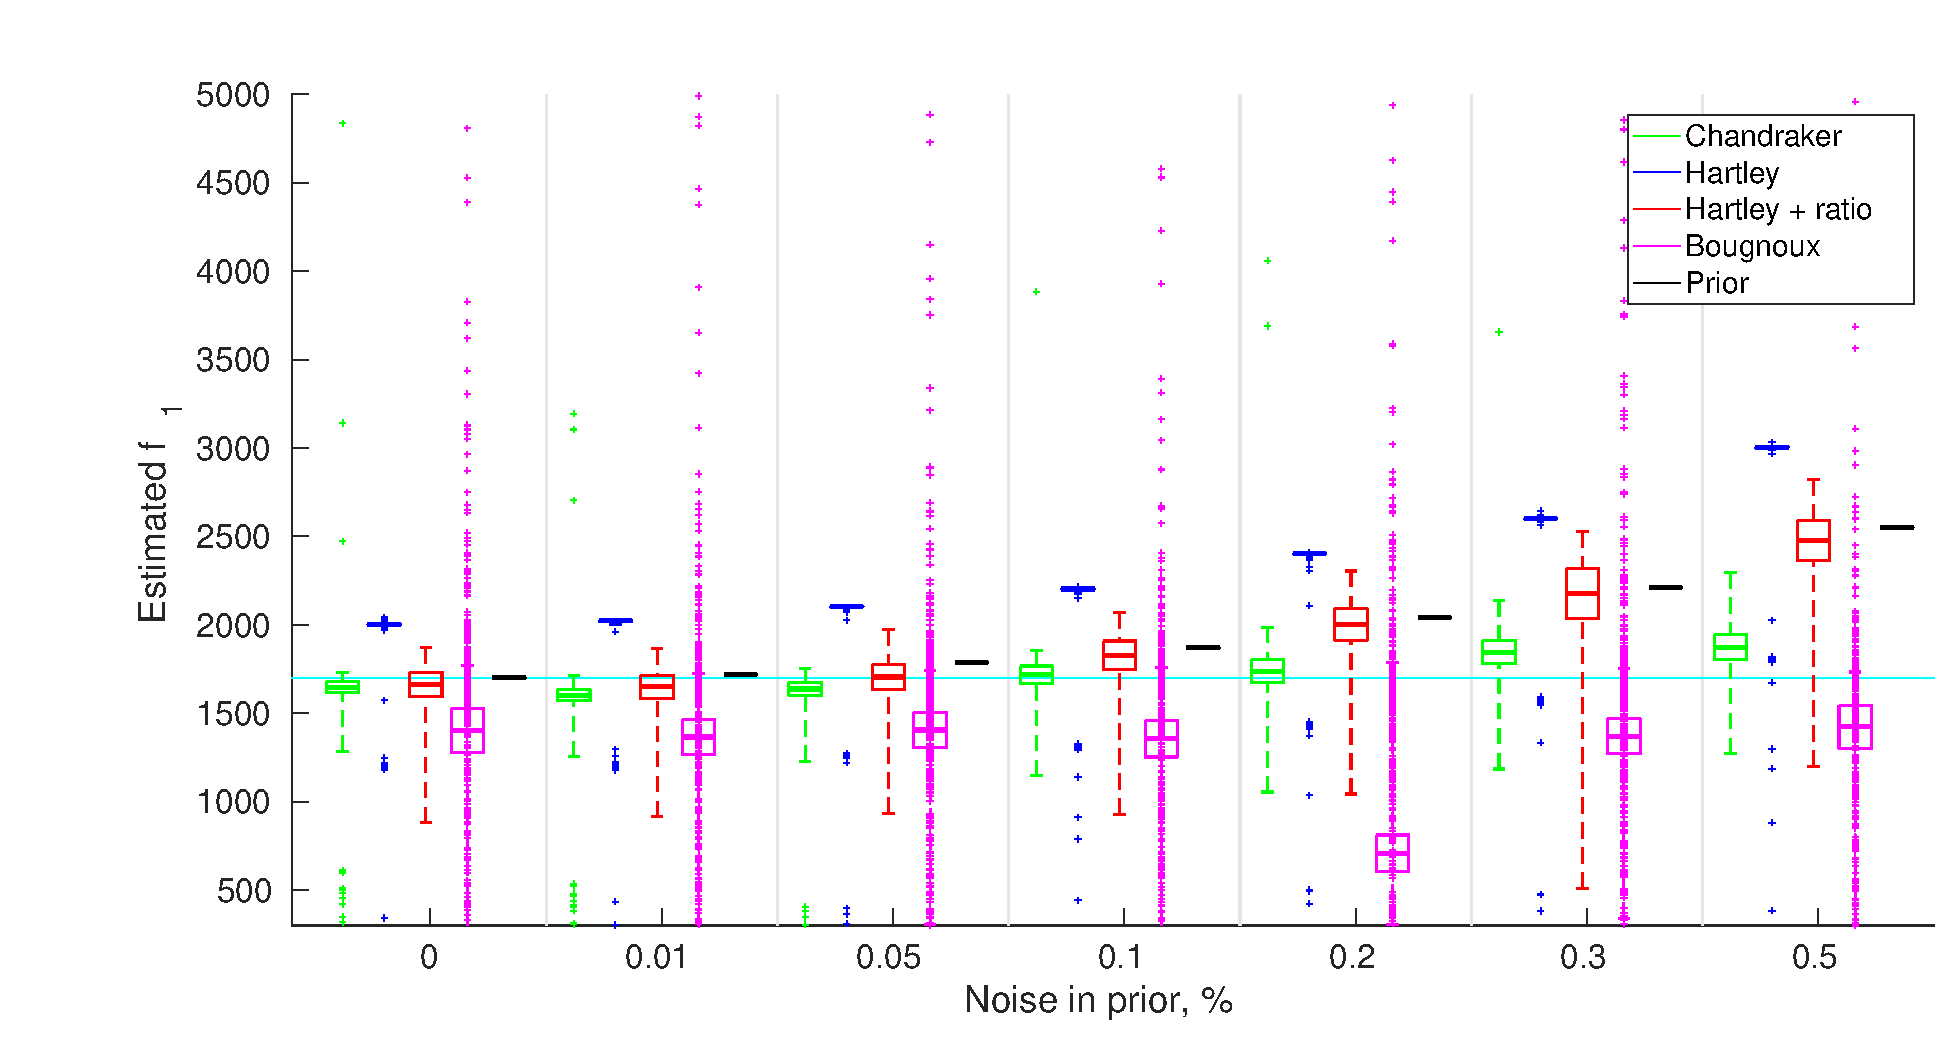
\includegraphics[width=\linewidth]{opt_comp_f1.eps}
    \caption[Comparison of the focal length methods. f1]{A comparison of the methods for computing focal lengths from point correspondences.  The ground truth focal length $f_1$ was 1700 (shown in cyan), and the relative noise (axis $x$) was added to it to produce priors, i. e., the priors were: 1700, 1717, 1785, 1870, 2040, 2210, 2550.  The ground truth principal points were both (10,20), and the prior principal points were $(0, 0)$. The number of correspondences used was 7, and the level of noise $\sigma$ was equal to 1. The weights on principal point priors were 10 times smaller than weights on focal lengths priors. The term enforcing the ratio of focal length in our modified version has the same weight as the terms for the focal lengths themselves.}
    \label{opt_comp_f1}
  \end{center}
\end{figure}



\begin{figure}[h!]
  \begin{center}
    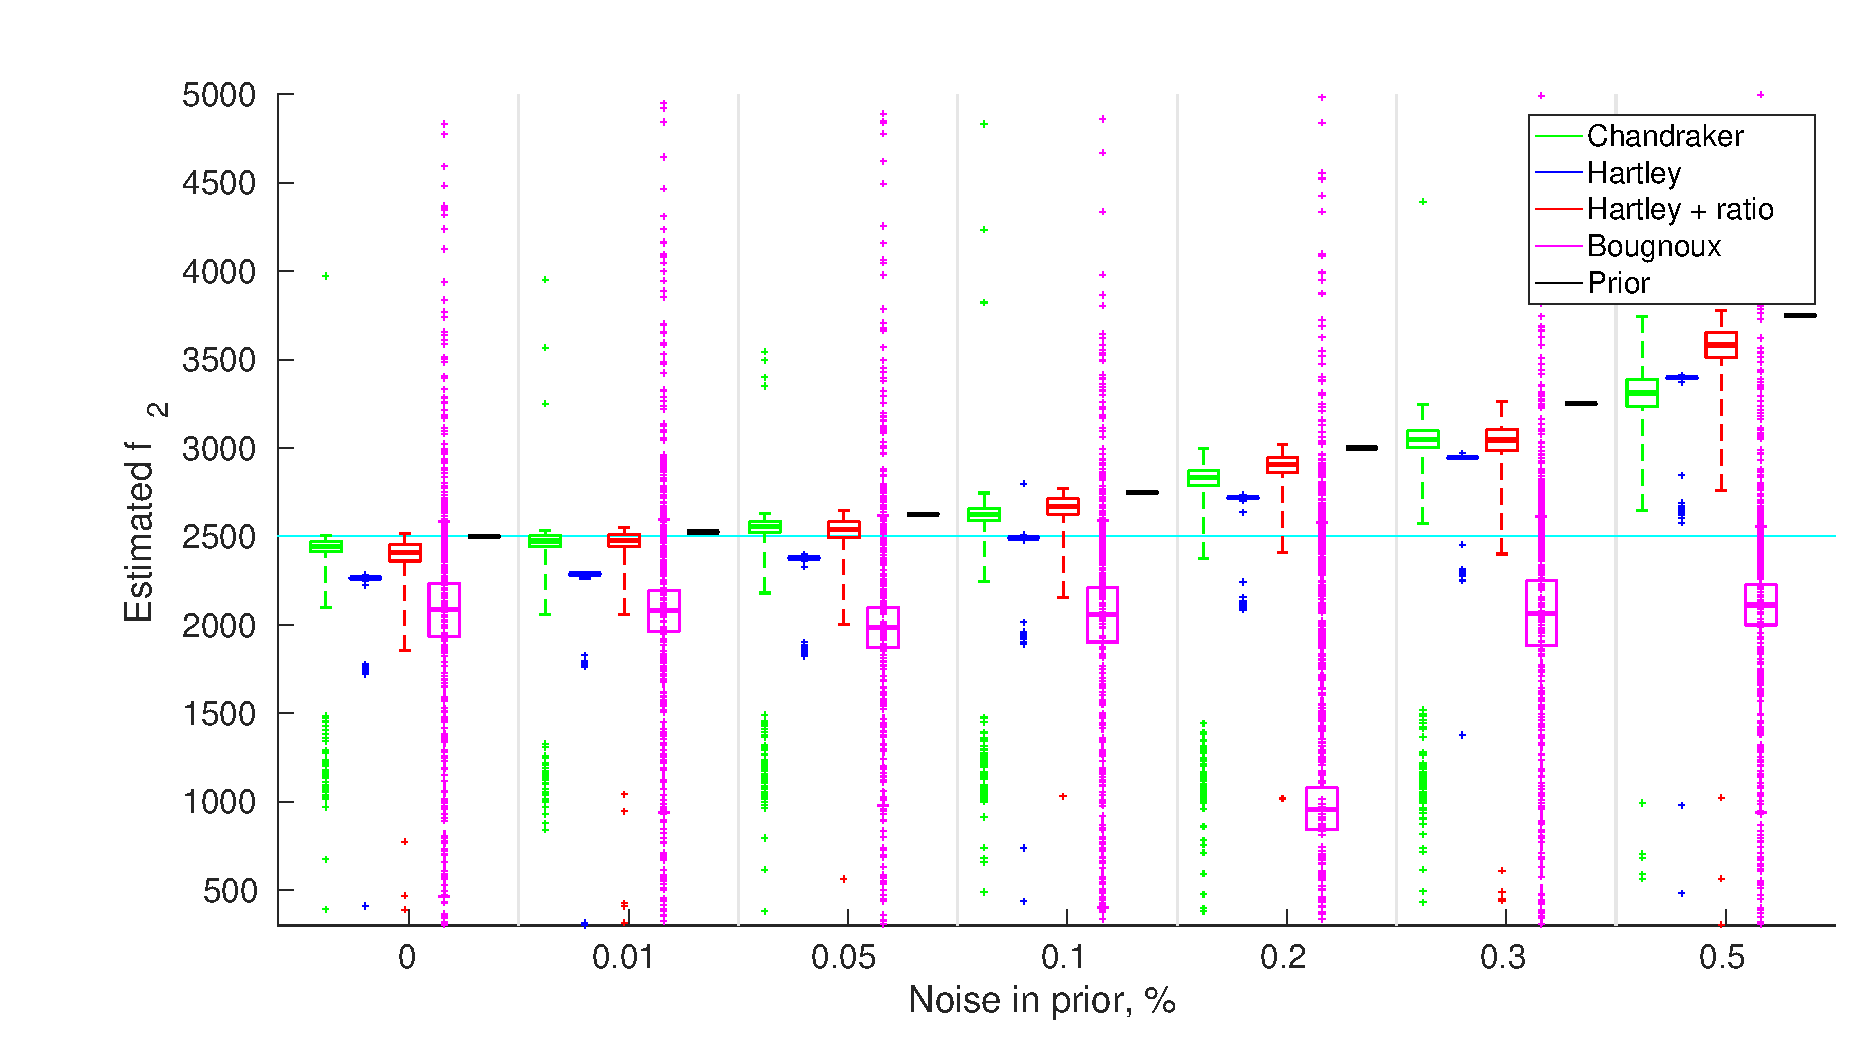
\includegraphics[width=\linewidth]{opt_comp_f2.eps}
    \caption[Comparison of the focal length methods. f1]{A comparison of the methods for computing focal lengths from point correspondences.  The ground truth focal length $f_2$ was 2500 (shown in cyan), and the relative noise (axis $x$) was added to it to produce priors, i. e., the priors were: 2500, 2525, 2625, 2750, 3000, 3250, 3750.}
    \label{opt_comp_f2}
  \end{center}
\end{figure}

\section{Conclusions}
We conclude that the fact that focal length ratio $r= f_2\slash f_1$ is robust can be used to construct more efficient algorithms. We show two examples of modifications to existing algorithms where we explicitly use a ratio estimation to improve the accuracy of the focal lengths computation. We show that using prior knowledge about focal length considerably bigger amounts of noise could be treated.

\chapter{Conclusions}

In this work, we have focused on the methods of computing the focal length from point correspondences. 

In Chapter~\ref{seq:basic} we surveyed the existing methods for this task, as well as the basic concepts needed for understanding them. We provided specific degeneracies of the methods and other cases where they might fail.
 
In Chapter~\ref{seq:analysis} we analyzed the performance of the different methods for computing the focal length. We have revealed several trends which these algorithms exhibit. Firstly, the error of the focal length estimation declines rapidly with growing number of correspondences. Secondly, with growing number of correspondences, the number of imaginary focal length estimates also declines. A conclusion can be made that the standard methods work fairly well for scenes where a sufficient number of inlier correspondences may be found.

We compared the performance of minimal solvers that use or don't use the rank constraint (Eq.~\ref{eq:rank}). Our results found that using rank constraint isneficial for the performance, however, such a solver might produce a larger fraction of imaginary estimates.

We found that  the computation of the ratio of focal length $r= f_2 \slash f_1$ by the Bougnoux formula~\cite{Bougnoux} is more robust than the computation of $f_1$ or $f_2$ alone. Interestingly, this robustness is preserved even when both focal length estimates are imaginary.

We furthermore assessed the performance of the methods in  degenerate situations. The results showed that for bigger levels of noise in image measurements the effect of the degeneracies significantly decreases. Specifically, the effects of the intersecting optical axes degeneracy was shown to be mild under 1 pixel noise in image measurements already.


In Chapter~\ref{seq:algeom} we analyzed the problem of computing focal length using the techniques of algebraic geometry. We have shown how the Bougnoux formula may be derived with these techniques and give two new formulae for computing camera focal length from a fundamental matrix, as well as one formula for the ratio of the focal length.  We have shown that using the right formula helps avoiding a known degeneracy. Specifically, the degeneracy where the plane defined by the baseline and the optical axis of one camera is perpendicular to the plane defined by the baseline and optical axis of the other camera, and where Bougnoux~(\cite{Bougnoux}) formula fails can in some cases be avoided. The degeneracy reduces to the case where all three formulae fail.

In Chapter~\ref{seq:thenew} we suggested improvements to the existing methods using our suggestion that computation of the ratio of focal length $r= f_2 \slash f_1$ is more robust than computation of $f_1$ or $f_2$ alone. We have shown that this fact indeed may improve performance of a solver. We suggested a modification to the solver of~\cite{HartleyPriors} and demonstrated an improvement in focal length estimation quality over the original method. Finally, we presented a survey of optimization methods for focal lengths computing and have shown that the optimization methods using prior focal length information may exhibit robust performance even under big amounts of noise in image measurements.

\appendix

\chapter{Contents of the enclosed CD}

\dirtree{%
 .1 /.
   .2 RobustFocal \DTcomment{\begin{minipage}[t]{8cm}folder with the all files of the thesis\end{minipage}}.
     .3 results \DTcomment{\begin{minipage}[t]{8cm}folder containing graphs that are included in the thesis\end{minipage}}.
       .4 \vdots.
     .3 lib \DTcomment{\begin{minipage}[t]{8cm}folder with auxiliary files required for the experiments\end{minipage}}.
       .4 generated\_solvers \DTcomment{\begin{minipage}[t]{8cm}solvers generated for the work using automatic generator~\cite{generator}\end{minipage}}.
        .5 \vdots.
       .4 utils \DTcomment{\begin{minipage}[t]{8cm}utility scripts\end{minipage}}.
        .5 \vdots.
       .4 geometry \DTcomment{\begin{minipage}[t]{8cm}geometrical utility scripts\end{minipage}}.
        .5 \vdots.
       .4 scene\_generator \DTcomment{\begin{minipage}[t]{8cm}scripts that generate a sample scene with points and cameras\end{minipage}}.
        .5 \vdots.
     .3 data \DTcomment{\begin{minipage}[t]{8cm}folder with synthetic 
     data generated for the experiments\end{minipage}}.
       .4 \vdots.
     .3 src \DTcomment{\begin{minipage}[t]{8cm}folder with the source files of the thesis\end{minipage}}.
       .4 analysis\_experiments \DTcomment{\begin{minipage}[t]{8cm}folder containing experiments for Chapter~\ref{seq:algeom}. \end{minipage}}.
        .5 \vdots.
       .4 algeom\_experiments \DTcomment{\begin{minipage}[t]{8cm}folder containing experiments for Chapter~\ref{seq:algeom}. \end{minipage}}.
        .5 \vdots.
       .4 thenew\_experiments \DTcomment{\begin{minipage}[t]{8cm}folder containing experiments for Chapter~\ref{seq:thenew}. \end{minipage}}.
        .5 \vdots.
       .4 geometry \DTcomment{\begin{minipage}[t]{8cm}folder containing geometrical functions written for the project. \end{minipage}}.
        .5 \vdots.
       .4 utils \DTcomment{\begin{minipage}[t]{8cm}folder containing utility functions written for the project. \end{minipage}}.
        .5 \vdots.
       .4 paths.m \DTcomment{\begin{minipage}[t]{8cm}script which add all required paths to the MAT\-LAB environment \end{minipage}}.
       .4 toy.m \DTcomment{\begin{minipage}[t]{8cm}script which runs a toy example of the focal length computation \end{minipage}}.
}

\bibliographystyle{plain}
\bibliography{citations}{}

\end{document}
